%===============================================================================
% LaTeX sjabloon voor de bachelorproef toegepaste informatica aan HOGENT
% Meer info op https://github.com/HoGentTIN/latex-hogent-report
%===============================================================================

\documentclass[dutch,dit,thesis]{hogentreport}

% TODO:
% - If necessary, replace the option `dit`' with your own department!
%   Valid entries are dbo, dbt, dgz, dit, dlo, dog, dsa, soa
% - If you write your thesis in English (remark: only possible after getting
%   explicit approval!), remove the option "dutch," or replace with "english".

\usepackage{lipsum} % For blind text, can be removed after adding actual content

%% Pictures to include in the text can be put in the graphics/ folder
\graphicspath{{../graphics/}}

%% For source code highlighting, requires pygments to be installed
%% Compile with the -shell-escape flag!
%% \usepackage[chapter]{minted}
%% If you compile with the make_thesis.{bat,sh} script, use the following
%% import instead:
\usepackage[chapter,outputdir=../output]{minted}
\usemintedstyle{solarized-light}

%% Formatting for minted environments.
\setminted{%
    autogobble,
    frame=lines,
    breaklines,
    linenos,
    tabsize=4
}

%% Ensure the list of listings is in the table of contents
\renewcommand\listoflistingscaption{%
    \IfLanguageName{dutch}{Lijst van codefragmenten}{List of listings}
}
\renewcommand\listingscaption{%
    \IfLanguageName{dutch}{Codefragment}{Listing}
}
\renewcommand*\listoflistings{%
    \cleardoublepage\phantomsection\addcontentsline{toc}{chapter}{\listoflistingscaption}%
    \listof{listing}{\listoflistingscaption}%
}

% Other packages not already included can be imported here

%%---------- Document metadata -------------------------------------------------
% TODO: Replace this with your own information
\author{Ernst Aarden}
\supervisor{Dhr. F. Van Houte}
\cosupervisor{Mevr. S. Beeckman}
\title[Optionele ondertitel]%
    {Titel van de bachelorproef}
\academicyear{\advance\year by -1 \the\year--\advance\year by 1 \the\year}
\examperiod{1}
\degreesought{\IfLanguageName{dutch}{Professionele bachelor in de toegepaste informatica}{Bachelor of applied computer science}}
\partialthesis{false} %% To display 'in partial fulfilment'
%\institution{Internshipcompany BVBA.}

%% Add global exceptions to the hyphenation here
\hyphenation{back-slash}

%% The bibliography (style and settings are  found in hogentthesis.cls)
\addbibresource{bachproef.bib}            %% Bibliography file
\addbibresource{../voorstel/voorstel.bib} %% Bibliography research proposal
\defbibheading{bibempty}{}

%% Prevent empty pages for right-handed chapter starts in twoside mode
\renewcommand{\cleardoublepage}{\clearpage}

\renewcommand{\arraystretch}{1.2}

%% Content starts here.
\begin{document}

%---------- Front matter -------------------------------------------------------

\frontmatter

\hypersetup{pageanchor=false} %% Disable page numbering references
%% Render a Dutch outer title page if the main language is English
\IfLanguageName{english}{%
    %% If necessary, information can be changed here
    \degreesought{Professionele Bachelor toegepaste informatica}%
    \begin{otherlanguage}{dutch}%
       \maketitle%
    \end{otherlanguage}%
}{}

%% Generates title page content
\maketitle
\hypersetup{pageanchor=true}

%%=============================================================================
%% Voorwoord
%%=============================================================================

\chapter*{Woord vooraf}%
\label{ch:voorwoord}

Voor u ligt mijn bachelorproef over het gebruik van semi- en self-supervised learningtechnieken voor objectdetectie op sonarbeelden. Dit onderzoek richt zich op de vraag of dergelijke technieken het labelproces kunnen versnellen zonder significant verlies in nauwkeurigheid. Het doel is een efficiëntere methode ontwikkelen voor het verwerken van sonardata. \\

Mijn interesse in dit onderwerp ontstond vanuit een combinatie van mijn passie voor machine learning en de uitdagingen die ik tijdens mijn stage tegenkwam. Het verwerken en labelen van sonardata bleek een tijdrovend en arbeidsintensief proces te zijn. Dit gaf me het idee om innovatieve methoden te verkennen om dit te optimaliseren. Semi- en self-supervised learning boden een veelbelovende oplossing, en ik was benieuwd of deze technieken in de praktijk daadwerkelijk een verschil konden maken. \\

Het schrijven van deze bachelorproef was een enorm leerzaam, maar uitdagend proces, waarin ik veel heb bijgeleerd over machine learning en de praktische toepassingen ervan binnen de industrie. Dit onderzoek zou niet mogelijk zijn geweest zonder de steun en begeleiding van verschillende mensen, aan wie ik graag mijn dank wil uitspreken. \\

Allereerst wil ik mijn promotor, mevr. Chantal Teerlinck, bedanken voor de goede begeleiding, feedback en inzichten tijdens dit traject. Haar ervaring en ondersteuning hebben me geholpen om dit onderzoek in de juiste richting te sturen. Daarnaast wil ik mijn co-promotor, mevr. Stefanie Duyck, bedanken voor haar betrokkenheid, kennis en praktische inzichten vanuit de bedrijfswereld, wat een belangrijke meerwaarde vormde voor dit onderzoek. \\

Ook wil ik mijn dank uitspreken aan Exail Robotics Belgium voor de kans om mijn bachelorproef binnen hun organisatie uit te voeren. De toegang tot zeer waardevolle resources en de begeleiding vanuit het team hebben een cruciale rol gespeeld in het realiseren van dit onderzoek. Tot slot wil ik mijn familie en vrienden bedanken voor hun steun en aanmoediging gedurende mijn studietraject. \\

Ik hoop dat deze bachelorproef een bijdrage kan leveren binnen het domein van objectdetectie op sonarbeelden en machine learning in het algemeen.
%%=============================================================================
%% Samenvatting
%%=============================================================================

% TODO: De "abstract" of samenvatting is een kernachtige (~ 1 blz. voor een
% thesis) synthese van het document.
%
% Een goede abstract biedt een kernachtig antwoord op volgende vragen:
%
% 1. Waarover gaat de bachelorproef?
% 2. Waarom heb je er over geschreven?
% 3. Hoe heb je het onderzoek uitgevoerd?
% 4. Wat waren de resultaten? Wat blijkt uit je onderzoek?
% 5. Wat betekenen je resultaten? Wat is de relevantie voor het werkveld?
%
% Daarom bestaat een abstract uit volgende componenten:
%
% - inleiding + kaderen thema
% - probleemstelling
% - (centrale) onderzoeksvraag
% - onderzoeksdoelstelling
% - methodologie
% - resultaten (beperk tot de belangrijkste, relevant voor de onderzoeksvraag)
% - conclusies, aanbevelingen, beperkingen
%
% LET OP! Een samenvatting is GEEN voorwoord!

%%---------- Samenvatting -----------------------------------------------------
% De samenvatting in de hoofdtaal van het document

\chapter*{\IfLanguageName{dutch}{Samenvatting}{Abstract}}

Sinds de opkomst en popularisatie van AI-modellen is data steeds een cruciale resource geweest. Voor simpele modellen is de benodigde data vaak ook simpel van vorm en is er (relatief) weinig van nodig om een performant en goed werkend model te creëren. Echter stijgen de data-requirements voor grotere en complexere modellen exponentieel. De benodigde data om een objectdetectiemodel voor sonardata te trainen zorgt voor moeilijkheden: dit soort datasets zijn online niet off-the-shelf beschikbaar en zijn dus zeer tijdrovend en kostbaar om te maken. De hoofdvraag van dit onderzoek is daarom: Op welke manieren kan het gebruik van semi- of self-supervised learning het labelproces versnellen zonder een significant verlies in nauwkeurigheid? Door verschillende technieken toe te passen, zal een pretraining-strategie ontwikkeld worden die gebruikmaakt van ongelabelde data om representaties aan te leren. Vervolgens zal onderzocht worden hoeveel gelabelde data nodig is om een goed presterend detectiemodel te trainen. Het doel is een methodologie te ontwikkelen die de afhankelijkheid van handmatig gelabelde data minimaliseert, terwijl de prestaties van het detectiemodel behouden blijven. De resultaten kunnen bijdragen aan efficiëntere workflows voor data-analyse in sonarbeeldvorming en andere domeinspecifieke contexten.


%---------- Inhoud, lijst figuren, ... -----------------------------------------

\tableofcontents

% In a list of figures, the complete caption will be included. To prevent this,
% ALWAYS add a short description in the caption!
%
%  \caption[short description]{elaborate description}
%
% If you do, only the short description will be used in the list of figures

\listoffigures

% If you included tables and/or source code listings, uncomment the appropriate
% lines.
\listoftables

\listoflistings

% Als je een lijst van afkortingen of termen wil toevoegen, dan hoort die
% hier thuis. Gebruik bijvoorbeeld de ``glossaries'' package.
% https://www.overleaf.com/learn/latex/Glossaries

%---------- Kern ---------------------------------------------------------------

\mainmatter{}

% De eerste hoofdstukken van een bachelorproef zijn meestal een inleiding op
% het onderwerp, literatuurstudie en verantwoording methodologie.
% Aarzel niet om een meer beschrijvende titel aan deze hoofdstukken te geven of
% om bijvoorbeeld de inleiding en/of stand van zaken over meerdere hoofdstukken
% te verspreiden!

%%=============================================================================
%% Inleiding
%%=============================================================================

\chapter{Inleiding}%
\label{ch:inleiding}

Objectdetectie heeft de afgelopen jaren enorme vooruitgang geboekt dankzij de opkomst van deep learning en de beschikbaarheid van grote, gelabelde datasets. In domeinen zoals computervisie, waar overvloedige trainingsdata gemakkelijk toegankelijk is, hebben deze technieken indrukwekkende prestaties bereikt. Echter beschikken niet alle vakgebieden over dergelijke datasets. In gespecialiseerde domeinen, zoals sonarbeeldanalyse, is gelabelde data schaars, wat het trainen van nauwkeurige detectiemodellen bemoeilijkt. Dit onderzoek richt zich op het verkennen van alternatieve leermethoden die deze afhankelijkheid van handmatige annotatie kunnen verminderen, zonder in te boeten op de prestaties van het model.

\section{Probleemstelling}%
\label{sec:probleemstelling}

Om een model te trainen dat met hoge precisie objecten in afbeeldingen kan herkennen en aanduiden, is een grote hoeveelheid gelabelde data nodig. Dit betekent dat naast de afbeeldingen zelf ook informatie over de positie van het object op de afbeelding beschikbaar moet zijn. Na de training is het de bedoeling dat het model deze informatie kan voorspellen op ongekende afbeeldingen. Sinds de opkomst van objectdetectie binnen het veld van machine learning zijn verschillende datasets openbaar beschikbaar gesteld die vrij gebruikt mogen worden om een dergelijk model te trainen. Dit geldt echter niet voor sonardata, om meerdere redenen. \\

Allereerst is objectdetectie op sonarbeelden een nicheprobleem. Hierdoor beschikken slechts weinig mensen over de kennis en expertise om zo’n dataset samen te stellen en, nog belangrijker, correct te annoteren. Daarnaast is er het – misschien nog grotere – probleem van de data zelf. Dit type gegevens kan niet eenvoudig met een camera worden verzameld; er is een gespecialiseerde sonarinstallatie voor nodig. Voor bedrijven is de aanschaf van zo’n installatie vaak weinig rendabel. Wel worden dergelijke systemen gebruikt voor militaire doeleinden, maar de data die hieruit voortkomt, is om veiligheidsredenen vrijwel altijd geclassificeerd. \\

De probleemstelling is dus tweeledig: er is weinig gelabelde sonardata voor objectdetectie beschikbaar, en het annoteren van een dergelijke dataset is moeilijk, tijdrovend en kostbaar.

\section{Onderzoeksvraag}%
\label{sec:onderzoeksvraag}

Om kosten en tijd te besparen, zou het dus ideaal zijn als er zo min mogelijk annotatie van de dataset nodig is. Bij supervised learning is dit echter nagenoeg onmogelijk, aangezien het model juist getraind wordt op basis van het verband tussen de afbeelding en de annotatie. Er bestaan echter veelbelovende alternatieven, zoals semi- en self-supervised learning, om dit probleem te overbruggen. Deze technieken maken gebruik van ongesuperviseerde data om representaties te leren en beperken zo de afhankelijkheid van gelabelde data. Moderne semi- en self-supervised methoden hebben indrukwekkende resultaten laten zien in domeinen zoals computer vision, maar hun toepassing op domeinspecifieke datasets, zoals sonar, is nog relatief onbekend terrein. \\

De hoofdvraag van dit onderzoek is daarom: Op welke manieren kan het gebruik van semi- of self-supervised learning het labelproces versnellen zonder een significant verlies in nauwkeurigheid?

\section{Onderzoeksdoelstelling}%
\label{sec:onderzoeksdoelstelling}

Het onderzoek verwacht aan te tonen dat semi- en self-supervised learning effectief kunnen worden ingezet om het labelproces bij sonarobjectdetectie aanzienlijk te versnellen. Door technieken zoals SimCLR, BYOL, Pseudo-Labeling en FixMatch te gebruiken voor pre-training, wordt verwacht dat het model sterke representaties leert van ongesuperviseerde sonardata, waardoor de behoefte aan grootschalige gelabelde datasets afneemt. Daarnaast zal een analyse inzicht geven in de minimale hoeveelheid gelabelde data die nodig is om vergelijkbare of betere prestaties te behalen dan met volledig supervised-learning methoden. \\

Dit resulteert in een efficiëntere en kosteneffectieve aanpak voor objectdetectie in sonarbeelden, zonder verlies van nauwkeurigheid, en biedt een waardevolle methodologie voor verdere toepassingen in domeinen waar gelabelde data schaars is.

\section{Opzet van deze bachelorproef}%
\label{sec:opzet-bachelorproef}

De rest van deze bachelorproef is als volgt opgebouwd: \\

In Hoofdstuk~\ref{ch:stand-van-zaken} wordt een overzicht gegeven van de stand van zaken binnen het onderzoeksdomein, op basis van een literatuurstudie. \\

In Hoofdstuk~\ref{ch:methodologie} wordt de methodologie toegelicht en worden de gebruikte onderzoekstechnieken besproken om een antwoord te kunnen formuleren op de onderzoeksvragen. \\

In Hoofdstuk~\ref{ch:data} begint het eigenlijke onderzoek. In deze eerste fase wordt een beschikbare dataset gepreprocessed voor gebruik in volgende hoofdstukken. \\

In Hoofdstuk~\ref{ch:implementatie} worden de verschillende modellen die vooraf uitgekozen zijn uit de verschillende categorieën geïmplementeerd in Python met behulp van Keras en TensorFlow. \\

In Hoofdstuk~\ref{ch:training-optimalisatie} worden de geïmplementeerde modellen getraind op de gepreprocesseerde dataset. Daarnaast worden de modellen geoptimaliseerd met behulp van hyperparameter tuning en andere technieken. \\

In Hoofdstuk~\ref{ch:evaluatie-modellen} worden de getrainde modellen geëvalueerd op basis van verschillende criteria. Er wordt een vergelijking gemaakt tussen -- onder andere -- de performantie van elk model en er wordt bepaald welk model de beste is. \\

In Hoofdstuk~\ref{ch:evaluatie-resultaten} wordt de praktische toepassing van de verschillende modellen geëvalueerd. Ook zullen enkele experts in sonaranalyse de bruikbaarheid van de resultaten beoordelen en aanbevelingen geven voor verdere verbeteringen. \\

In Hoofdstuk~\ref{ch:conclusie}, tenslotte, wordt de conclusie gegeven en een antwoord geformuleerd op de onderzoeksvragen. Daarbij wordt ook een aanzet gegeven voor toekomstig onderzoek binnen dit domein.
\chapter{Stand van zaken}
\label{ch:stand-van-zaken}

\section{Inleiding}

Objectdetectie in domeinspecifieke contexten zoals sonarbeeldvorming wordt vaak gehinderd door een gebrek aan gelabelde data. Traditioneel vereisen gesuperviseerde modellen grote hoeveelheden handmatig gelabelde gegevens om effectieve detectie en classificatie te leren. Semi-supervised en self-supervised learning bieden echter veelbelovende alternatieven door gebruik te maken van grote hoeveelheden ongesuperviseerde data om representaties te leren. Deze literatuurstudie bespreekt de huidige technieken en hun toepassing, met een specifieke focus op de unieke uitdagingen van sonardata.

% Objectdetectie in sonarafbeeldingen
\section{Objectdetectie in sonarafbeeldingen}

\subsection{Definitie en gebruik op sonarafbeeldingen}

Objectdetectie is een tak binnen het domein van computer vision dat gericht is op het identificeren en lokaliseren van objecten binnen beelddata (zoals foto's en video's). Dit wordt gebruikt in verschillende domeinen, zoals beveiligingssystemen (bv. om inbrekers te detecteren) of de medische wereld (bv. om tumoren op te sporen). Door de jaren heen is objectdetectie aanzienlijk geëvolueerd dankzij de vooruitgang in deep learning en de grote beschikbaarheid van datasets met beeldmateriaal. \autocite{He_2016} \\

Objectdetectie combineert twee belangrijke zaken in computer vision: objectlokalisatie en objectclassificatie. Objectlokalisatie bepaalt de positie van objecten, meestal in de vorm van \glspl{bounding_box} \autocite{Tompson_2015}, terwijl objectclassificatie bepaalt tot welke categorie een gedetecteerd object behoort. Samen geeft dit de mogelijkheid tot het herkennen van verschillende soorten objecten op één foto. \\

Objectdetectie heeft vele toepassingen, ook in domeinen die misschien niet zo voor de hand liggend zijn. Één van deze specialisaties binnen de -- algemene -- objectdetectie is objectdetectie op sonardata. Dit domein is over de laatste jaren erg gegroeid, vooral onder invloed van buitenlandse dreigingen. Zo wordt sonarobjectdetectie gebruikt voor het opsporen van mijnen in zee om ze later onschadelijk te kunnen maken. Naast detectie van mijnen wordt   de techniek ook gebruikt voor verschillende soorten onderzoeken, zoals archeologisch en maritiem onderzoek. Bij deze verschillende toepassingen wordt natuurlijk telkens een kleine variatie op deze techniek gebruikt om telkens andere dingen op te sporen. \autocite{Wang_2024} \\

Traditioneel worden supervised-learning methoden gebruikt voor objectdetectie. Voorbeelden van populaire architecturen binnen dit domein zijn onder andere Faster \gls{rcnn}, \gls{yolo} en \gls{ssd}. \autocite{Redmon_2016} Omdat dit supervised-learning modellen zijn, presteren  ze uitstekend bij voldoende gelabelde data. De annotatiekosten en tijdsinvestering vormen echter een grote belemmering, vooral bij complexe datasets zoals sonar. Sonardata vereist namelijk gespecialiseerde kennis voor het labelen, wat de annotatie nog uitdagender maakt. \autocite{Long_2015} \\

Deze supervised objectdetectietechnieken vallen onder te verdelen in grofweg twee grote categorieën. Enerzijds zijn er de zogenaamde \emph{single-shot detectors}, anderzijds heb je de \emph{two-stage detectors}. Deze categorieën zijn gebaseerd op hoeveel keer de afbeelding door het netwerk gaat. Bij single-shot detectors gaat de afbeelding slechts één keer door het netwerk, bij two-stage detectors -- logischerwijs -- twee keer. \autocite{Carranza_Garcia_2020} \\

Één van de eerste succesvolle toepassingen van deep learning binnen het domein van objectdetectie gebeurde in een bekend artikel van \textcite{Girshick_2013}. In dit artikel stelden de auteurs de \gls{rcnn}-architectuur voor. Deze veelbelovende architectuur behaalde een \gls{map} van 30\% meer dan de vorige topscore op een bekende publieke dataset (\acrshort{voc} 2012).

\subsubsection{Single-shot objectdetectie}

Zoals hierboven vermeld, is een single-shot detector een model waarbij de afbeelding slechts één keer door het netwerk gaat. Dit gebeurd door een \gls{cnn} te gebruiken dat zowel objectlocaties als bijbehorende classificaties voorspelt in één enkele \emph{pass}. Het voordeel van dit soort architectuur is dat ze zeer resource-efficiënt is, aangezien elke afbeelding slechts één keer behandeld wordt. Omwille van de efficiëntie, is deze architectuur dus uitermate geschikt voor real-time toepassingen zoals autonome voertuigen en bewakingssystemen. Een nadeel is echter dat het model niet altijd even precies is, aangezien het zowel locaties als klassen in één pass moet voorspellen. Vooral bij het detecteren van kleine objecten geeft dit een probleem. Om dit -- toch gedeeltelijk -- op te lossen, wordt soms gebruik gemaakt van meerdere schaalniveaus om objecten van verschillende groottes te detecteren, wat bijdraagt aan de robuustheid en precisie. \autocite{Carranza_Garcia_2020} \\

Zowel \gls{yolo} als \gls{ssd} zijn single-shot detectors. Deze architecturen worden verder besproken in latere secties hieronder.

\subsubsection{Two-stage objectdetectie}

Zoals de naam doet vermoeden, is two-stage objectdetectie een type objectdetectie waarbij de afbeelding twee keer door het netwerk gaat. Het resultaat is nog steeds een voorspelling van locaties en klassen, maar in plaats van in één keer -- zoals bij single-shot objectdetectie -- gebeurt de voorspelling nu in twee afzonderlijke stappen. Het resultaat van de eerste \emph{pass} is een set van \emph{proposals} -- voorstellen -- en mogelijke locaties van objecten. Daarna zorgt de tweede \emph{pass} voor een verfijning van deze voorstellen. Dit zorgt dan ook voor de uiteindelijke voorspellingen. Het voordeel van dit type objectdetectie is dat het veel preciezer is dan single-shot objectdetectie, aangezien de afbeelding twee keer geanalyseerd wordt. Het nadeel is dat deze approach veel resource-intensiever is. Het is dus zaak om een afweging te maken tussen de precisie van de voorspellingen en het verbruik van resources. \autocite{Carranza_Garcia_2020} \\

Over het algemeen wordt voor real-time applicaties single-shot objectdetectie gebruikt en voor cases waar de voorspellingen heel accuraat moeten zijn, wordt two-stage objectdetectie gebruikt. Een voorbeeld van een two-stage detector is de \gls{rcnn}-architectuur van \textcite{Girshick_2013}. Ook alle latere architecturen die hierop gebaseerd zijn, zijn two-stage detectors. Voorbeelden daarvan zijn Fast \gls{rcnn}, Faster \gls{rcnn} en Mask \gls{rcnn}. \autocite{Ren_2015}

\subsection{Meten van performantie binnen objectdetectie}

Gedurende dit onderzoek zal er gewerkt worden met verschillende soorten modellen en architecturen met elk hun sterktes en hun zwaktes. Het is de bedoeling dat al deze modellen vergeleken kunnen worden met elkaar om zo het best presterende model of de best presterende modellen te kunnen selecteren. Om dit te doen zijn er standaard metrieken nodig. Deze kunnen later (tijdens de trainingsfase) dan ook dienen als \gls{loss_functie}. Er zijn enorm veel verschillende metrieken om de performantie van objectdetectiemodellen te meten, maar twee van de bekendste en meest gebruikte zijn \gls{iou} en \gls{map}.

\subsubsection{Intersection over Union (IoU)}

\gls{iou} is een heel bekende metriek om de accuraatheid van de lokalisatie binnen objectdetectiemodellen te berekenen. Om de \gls{iou} te berekenen wordt gebruikt gemaakt van de echte \gls{bounding_box} en de voorspelde \gls{bounding_box}. Eerst wordt de overlappende oppervlakte (de doorsnede of \emph{intersection} in het Engels) van de twee \glspl{bounding_box} berekend. Daarna wordt de totale oppervlakte (de unie of \emph{union} in het engels) van de twee \glspl{bounding_box} berekend. \\

Door de doorsnede te delen door de unie krijgt men een verhouding van de overlappende oppervlakte tot de totale oppervlakte. Dit geeft een goede indicatie van hoe dicht de voorspelde \gls{bounding_box} bij de echte \gls{bounding_box} ligt. Een lagere \gls{iou}-score duidt op een betere prestatie, aangezien de voorspelde \gls{bounding_box} niet dan weinig afwijkt van de echte \gls{bounding_box}. \autocite{Rezatofighi_2019}

\begin{figure}[H]
    \centering
    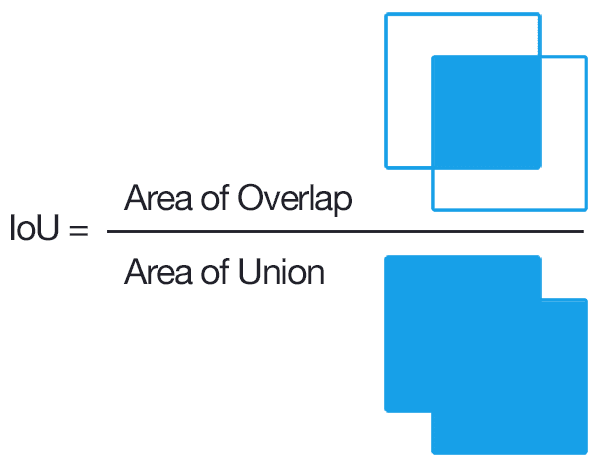
\includegraphics[width=0.5\textwidth]{iou_equation.png}
    \caption[Voorstelling van IoU.]{\label{fig:iou_equation}Formule en visuele voorstelling van de \acrfull{iou}. \autocite{Rosebrock_2016}}
\end{figure}

\subsubsection{mean Average Precision (mAP)}

Een andere -- zeer bekende -- metriek is de \acrfull{map}. Ze beoordeelt de nauwkeurigheid van een model op basis van zowel \gls{precision} als \gls{recall}. Het wordt berekend door de gemiddelde precisie (of \emph{average precision}, AP) over alle klassen en \gls{iou} drempels te bepalen. AP wordt verkregen door de oppervlakte onder de precisie-recallcurve van een specifieke klasse te berekenen door hem te integreren, en \gls{map} is vervolgens het gemiddelde van deze waarden over alle klassen. Een hogere mAP-score duidt op betere prestaties van een objectdetectiemodel, omdat het aangeeft hoe goed het model objecten correct detecteert en classificeert. \autocite{Wang_2022}

\subsection{Typische uitdagingen bij sonarobjectdetectie}

Objectdetectie op sonarbeelden die gemaakt zijn onderwater wordt geconfronteerd met verschillende uitdagingen die de nauwkeurigheid en betrouwbaarheid van detecties beïnvloeden.

Ruis is een van de voornaamste obstakels bij sonarobjectdetectie. Onderwateromgevingen zijn inherent lawaaierig door factoren zoals luchtbellen, \glspl{thermocline} en biologische organismen, wat leidt tot significante ruis in sonarbeelden. Deze ruis bemoeilijkt het onderscheiden van echte objecten van artefacten typisch aan sonarbeelden, waardoor de betrouwbaarheid van de detecties afneemt. \autocite{Aubard_2024_Datasets} \\

Een andere uitdaging is de lage resolutie van sonarbeelden. In vergelijking met optische sensoren leveren sonars vaak beelden met beperkte detailweergave, wat de identificatie en classificatie van objecten moeilijker maakt. Deze beperking is vooral problematisch bij het detecteren van kleine of complexe objecten, waar detailniveau essentieel is voor nauwkeurige herkenning. \autocite{Lee_2018} \\

Daarnaast zorgen variërende omstandigheden in de onderwateromgeving voor extra complicaties. Factoren zoals veranderende waterdieptes, temperatuurverschillen, stromingen en de aanwezigheid van zwevende deeltjes kunnen de prestaties van sonarsystemen beïnvloeden. Deze dynamische omstandigheden kunnen leiden tot variaties in signaalsterkte en -kwaliteit, wat de consistentie van objectdetectie bemoeilijkt. \autocite{Valdenegro_Toro_2019} \\

Het overwinnen van deze uitdagingen vereist geavanceerde signaalverwerkingstechnieken en robuuste algoritmen die kunnen omgaan met ruis, lage resolutie en variabele omgevingsfactoren. Door voortdurende technologische innovaties en onderzoek kunnen de prestaties van sonarobjectdetectiesystemen worden verbeterd, wat leidt tot betrouwbaardere toepassingen in onderwateromgevingen.

\subsection{Overzicht van bestaande technieken}

Grofweg zijn er twee stromingen van objectdetectie op sonarafbeeldingen. Enerzijds zijn er de klassieke methoden en anderzijds zijn er de moderne deep learning-technieken. De klassieke methoden werden vooral gebruikt in een tijd waar grote, complexe neurale netwerken trainen onmogelijk was bij gebrek aan voldoende computerkracht, maar worden de dag van vandaag nog altijd gebruikt als pre-processing technieken voor de datasets waarmee de moderne neurale netwerken getraind worden. Deze klassieke methoden berusten enkel op statistische technieken om zo objecten in afbeeldingen te proberen detecteren. Specifiek zijn deze vooral gericht op het verbeteren van beeldkwaliteit en het onderscheiden van objecten van de achtergrond.

\subsubsection{Filtertechnieken}

Een voorbeeld van een klassieke methode zijn filtertechnieken. Deze worden toegepast om ruis in sonarafbeeldingen te verminderen en de beeldkwaliteit te verbeteren. Er bestaan immens veel verschillende soorten filters die elk geoptimaliseerd voor een specifiek doel. Een veelgebruikte filtermethode is het gebruik van adaptieve filters die zich aanpassen aan de lokale kenmerken van het beeld. Een voorbeeld hiervan is te vinden in een artikel van \textcite{Aridgides_1995}. Merk op dat dit inderdaad een relatief oude publicatie is, wat aantoont dat deze technieken al gebruikt werden toen deep learning-gebaseerde objectdetectie niet mogelijk was. \\

In dit artikel introduceren de auteurs een adaptieve filtertechniek die ontwikkeld is om mijnachtige doelen te onderscheiden van achtergrondruis in sonarbeelden. De filter onderdrukt achtergrondruis terwijl het de target behoudt. De procedure omvat vier stappen: het berekenen van een genormaliseerde gemiddelde target, het bepalen van de covariantiematrix van de achtergrondruis, het oplossen van normale vergelijkingen om een adaptief filter te verkrijgen en het toepassen van een 2D-filter op de gegevens. Dit algoritme bewijst dat, hoewel er geen gebruik gemaakt wordt van deep-learningtechnieken, ze toch complex kan zijn. De techniek heeft in verschillende testen prestaties geleverd die vergelijkbaar zijn met die van een ervaren sonaroperator. \\

Adaptieve filters worden ook vandaag de dag nog gebruikt, wat aangetoond wordt door een paper van \textcite{Lourey_2017}. Hierin wordt ook een filtertechniek beschreven die toegepast kan worden op \gls{cas} om interferentie van de directe transmissie en de echo van de target van elkaar te onderscheiden. Deze methode kan als effectieve pre-processing techniek gebruikt worden voor trainingsdata.

\subsubsection{Thresholding}

Naast filtering bestaan er nog andere klassieke methoden. Een \emph{straightforward}-aanpak is een simpele \emph{threshold}. Thresholding is een techniek waarbij pixelwaarden worden vergeleken met een bepaalde drempelwaarde om objecten van de achtergrond te scheiden. Een klassieke benadering is de Otsu-methode, die de interklassevariantie minimaliseert om een optimale drempelwaarde te bepalen. Deze methode wordt beschreven in een artikel van \textcite{Otsu_1979}.

\begin{figure}[H]
    \centering
    \begin{subfigure}{.5\textwidth}
        \centering
        \captionsetup{justification=centering}
        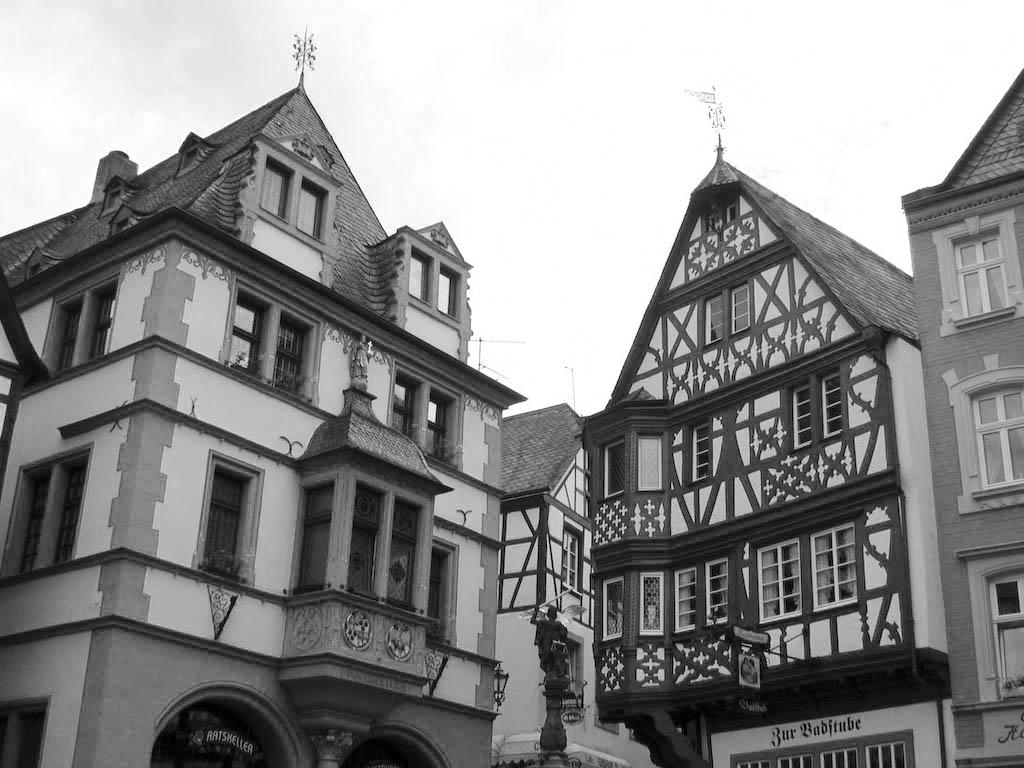
\includegraphics[width=0.9\linewidth]{img_pre_otsu.jpg}
        \caption[Afbeelding voor Otsu's thresholding]{Afbeelding voor Otsu's thresholding. \autocite{http//www.freephotos.lu/_2010}}
        \label{fig:img_pre_otsu}
    \end{subfigure}%
    \begin{subfigure}{.5\textwidth}
        \centering
        \captionsetup{justification=centering}
        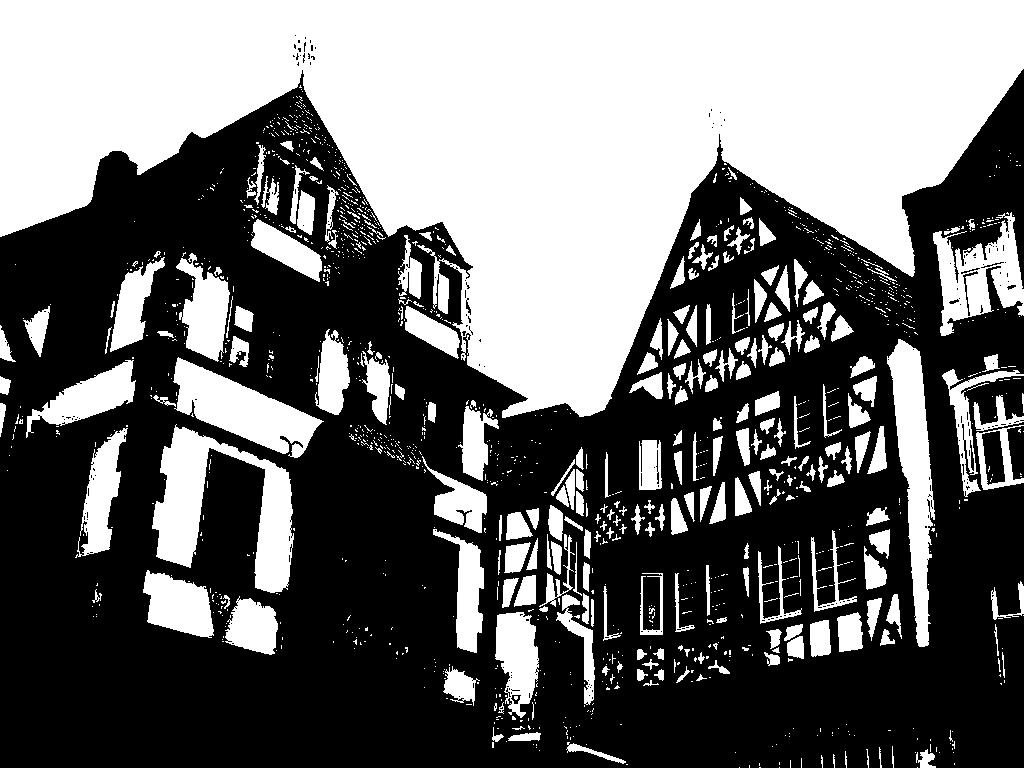
\includegraphics[width=0.9\linewidth]{img_post_otsu.jpg}
        \caption[Afbeelding na Otsu's thresholding]{Afbeelding na Otsu's thresholding. \autocite{Pikez33_2010}}
        \label{fig:img_post_otsu}
    \end{subfigure}
    \caption[Afbeelding voor en na Otsu's thresholding]{Afbeelding voor en na Otsu's thresholding}
    \label{fig:imgs_otsu}
\end{figure}

Hoewel deze techniek oorspronkelijk is ontwikkeld voor visuele beelden, is deze ook toegepast op sonarafbeeldingen, zoals besproken in verschillende artikels, waaronder dat van \textcite{Yuan_2016} en dat van \textcite{Dimitrova_Grekow_2017}. Ondanks zijn simpliciteit kan deze techniek aanzienlijke verbeteringen teweegbrengen. Dit wordt onder andere aangehaald in een paper van \textcite{Komari_Alaie_2018}. Deze paper onderzoekt objectdetectie met passieve sonar in de Perzische Golf. Aangezien deze binnenzee ondiep is, is er sprake van een hoge hoeveelheid fouten tijdens de detectie. Een bepaald soort adaptieve thresholding-techniek kon de \gls{precision} van hun objectdetectiemodel met 24\% verbeteren.

\subsubsection{Edge detection}

Edge detection is een andere klassieke techniek die wordt gebruikt om de contouren van objecten in sonarafbeeldingen te identificeren. \autocite{Torre_1986} Een bekende methode is de Canny edge detector, die randen detecteert door het maximaliseren van de gradiëntgrootte. Deze techniek komt als beste uit de vergelijkende studie van \textcite{Awalludin_2022}. \\

De Canny edge detector werkt in meerdere stappen om nauwkeurige en robuuste contourdetectie te realiseren. De eerste stap is Gaussian blurring, waarbij het beeld wordt vervaagd om ruis te verminderen en kleine details die geen significante randen vormen te onderdrukken. Vervolgens wordt de gradiënt van het beeld berekend met behulp van Sobel-operatoren in zowel de horizontale als verticale richting, waardoor de randen worden geaccentueerd. Daarna wordt non-maximum suppression toegepast, waarbij alleen de sterkste randen worden behouden en omliggende pixels met lagere gradiëntwaarden worden onderdrukt. De laatste stap is hysteresis thresholding, waarbij twee drempelwaarden worden gebruikt: pixels met een gradiëntsterkte boven de hoge drempel worden als randen geclassificeerd, terwijl pixels onder de lage drempel worden genegeerd. Pixels met tussenliggende waarden worden alleen als rand beschouwd als ze verbonden zijn met een sterke randpixel. Dankzij deze gefaseerde aanpak is de Canny-methode effectief in het detecteren van duidelijke randen, zelfs in ruisgevoelige omgevingen zoals sonarafbeeldingen. \autocite{Ding_2001} \\

Ook edge detection wordt vandaag de dag nog gebruikt om een grote bijdrage te leveren aan bijvoorbeeld segmentatiemodellen. Het onderzoek van \textcite{Priyadharsini_2019} gebruikt gespecialiseerde edge detection als pre-processing voor de data naar een objectdetectiemodel gaat. \\

Deze klassieke technieken vormen de basis voor objectdetectie in sonarafbeeldingen en hebben bijgedragen aan de ontwikkeling van meer geavanceerde methoden. Ze blijven relevant, vooral in situaties waarin resources beperkt zijn of wanneer eenvoud en interpretatie van het model belangrijk zijn. Ze worden tot op de dag van vandaag gebruikt als pre-processing stap, bijvoorbeeld. Doordat computerkracht steeds goedkoper en meer beschikbaar werd, wordt tegenwoordig vaak gekozen voor deep learning-oplossingen voor deze problemen. Er zijn gespecialiseerde architecturen ontwikkeld om objectdetectie uit te voeren. Hieronder worden er enkele besproken.

\subsubsection{YOLO}

\acrfull{yolo} is een deep learning-gebaseerde architectuur voor objectdetectie dat bekend staat om zijn snelheid en efficiëntie. Het werd voor het eerst geïntroduceerd in een artikel van \textcite{Redmon_2016} en is sindsdien één van de populairste algoritmes in computervisie. In tegenstelling tot traditionele detectiemethoden, waar objecten in meerdere stappen geanalyseerd worden, verwerkt YOLO een afbeelding in één enkele \emph{pass} van het neurale netwerk. Dit zorgt ervoor dat real-time objectdetectie mogelijk is, waardoor het bijzonder geschikt is voor toepassingen zoals autonome voertuigen, videobewaking en \gls{ar}.

\begin{figure}[H]
    \centering
    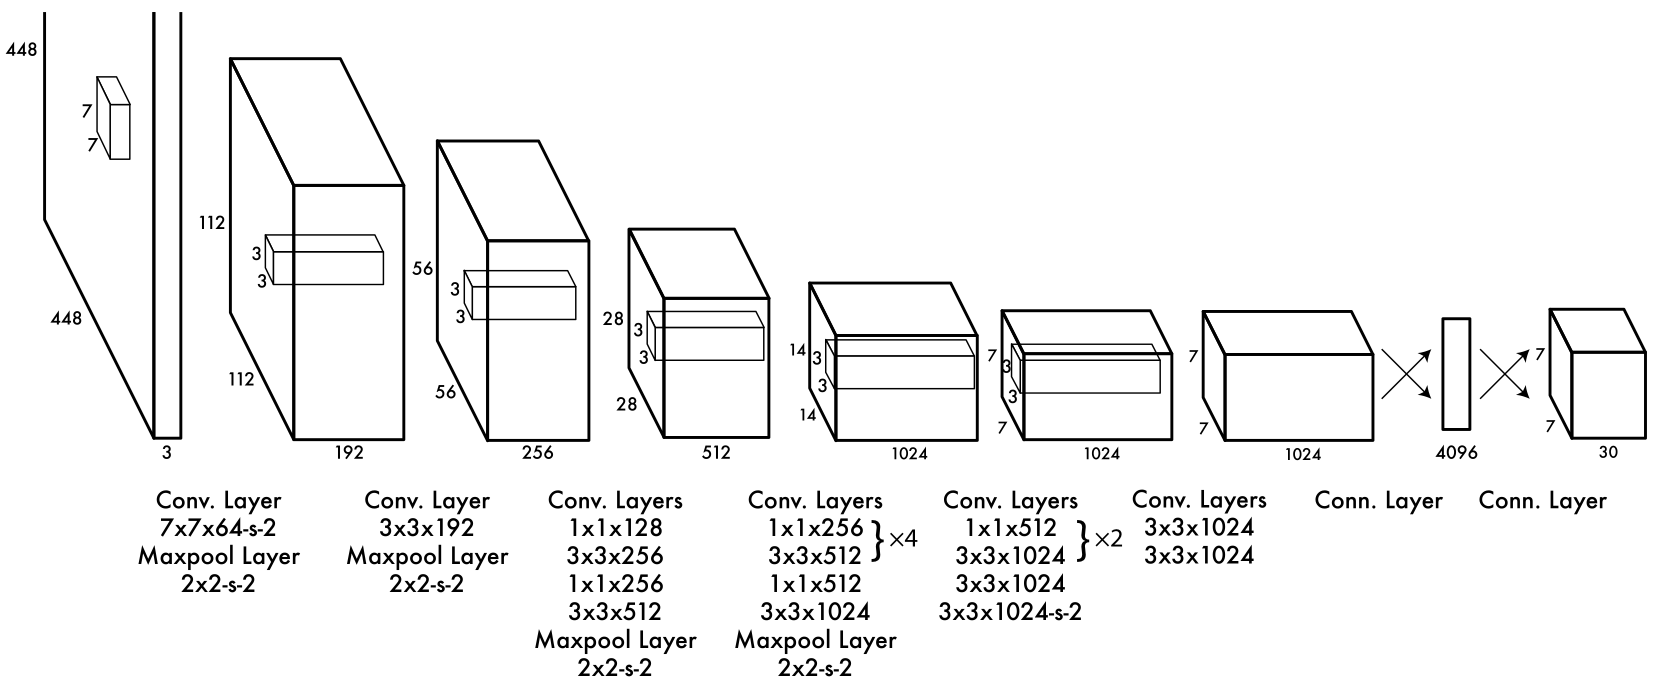
\includegraphics[width=\textwidth]{yolo_architecture.png}
    \caption[Originele YOLO-architectuur.]{\label{fig:yolo_architecture}Schematische voorstelling van de originele YOLO-architectuur. \autocite{Redmon_2016}}
\end{figure}

\gls{yolo} gebruikt een \gls{cnn} om objecten direct te lokaliseren en classificeren, wat bijdraagt aan de hoge nauwkeurigheid en snelheid van het model. De eerste versie van \gls{yolo} gebruikt ImageNet om de eerste 20 convolutionele lagen te pre-trainen. Het model wordt daarna omgezet om detectie uit te voeren, aangezien de combinatie van convolutionele lagen en fully-connected-lagen de performantie verhoogt. \autocite{Redmon_2016} De interne werking van \gls{yolo} kan opgesplitst worden in verschillende fasen. \\

Eerst en vooral wordt de invoerafbeelding opgesplitst in een $S \times S$ raster (bv. $7 \times 7$). Elke cel van dat raster is daarna verantwoordelijk voor het detecteren van objecten waarvan het midden zich in dat vak bevindt. Voor elke cel voorspelt \gls{yolo} meerdere \glspl{bounding_box}. Zo'n voorspelling van een \gls{bounding_box} bevat telkens 5 parameters (cf. \ref{fig:bounding_box}): 

\begin{itemize}
    \item $x$ en $y$: de gecentreerde coördinaten van het object binnen de cel in het raster.
    \item $w$ en $h$: de breedte en hoogte van het object, genormaliseerd ten opzichte van de afbeelding.
    \item De \gls{confidence_score}: de waarschijnlijkheid dat er daadwerkelijk een object in de box zit.
\end{itemize}

Naast het voorspellen van de \glspl{bounding_box} voorspelt het model ook de klasse van het object (bv. auto, hond, persoon, \dots) en de \gls{confidence_score} van deze classificatie. Echter zijn er vaak meerdere \glspl{bounding_box} die hetzelfde object detecteren. Daarom gebruikt \gls{yolo} \gls{nms} om overbodige detecties te verwijderen. Ten slotte genereert \gls{yolo} een lijst met gedetecteerde objecten, hun locaties en de waarschijnlijkheid van hun klassen. \autocite{Diwan_2022} \\

\gls{yolo} is sneller dan traditionele methoden zoals Faster R-CNN omdat het objectdetectie beschouwt als een enkel regressieprobleem. Dit betekent dat het model direct van ruwe pixels naar detecties gaat, zonder een apart proces voor regio-voorstel en classificatie. \\

Sinds de introductie van \gls{yolo} in de paper van \textcite{Redmon_2016} heeft het model aanzienlijke verbeteringen en evoluties doorgemaakt. De oorspronkelijke versie, \gls{yolo}v1, legde de basis met een enkelvoudige doorvoer voor objectdetectie, maar had beperkingen in nauwkeurigheid, vooral bij kleine objecten. \gls{yolo}v2 (ook wel \gls{yolo}9000) werd kort na de introductie van het originele \gls{yolo}-model geïntroduceerd in een paper van \textcite{Redmon_2016_YOLOv2}. De nieuwe versie werd ontwikkeld om sneller en accurater te zijn dan het originele model. Ook kon deze versie meer verschillende klassen onderscheiden. Daarnaast werd er gebruik gemaakt van een andere \emph{backbone}, namelijk Darknet-19 (wat zelf een variant is van VGGNet). Dit zijn de belangrijkste veranderingen:

\begin{itemize}
    \item Gebruik van een nieuwe \gls{loss_functie} die beter geschikt is voor objectdetectie.
    \item Gebruik van \gls{batch_normalisatie} om accuraatheid en stabiliteit te verhogen.
    \item Trainen op zelfde afbeeldingen met een verschillende schaal, hierdoor wordt het model beter in het herkennen van kleine objecten.
    \item Gebruik van zogenaamde \emph{anchor boxes}: dit zijn vooraf gedefinieerde \glspl{bounding_box} die helpen bij het detecteren van objecten in een afbeelding. Tijdens het trainen leert het model welke van deze \emph{anchor boxes} het beste passen bij de werkelijke objecten in de afbeelding.
\end{itemize}

\gls{yolo}v3 werd geïntroduceerd in een paper van \textcite{Redmon_2018}. Het doel van deze iteratie was opnieuw het verbeteren van de accuraatheid en de snelheid. Dit deden de onderzoekers door opnieuw een andere architectuur te gebruiken als \emph{backbone}. Dit keer gebruikten ze Darknet-53 (een variant van ResNet). Daarnaast werden de \emph{anchor boxes} aangepast zodat ze verschillende vormen en maten hadden (in tegenstelling tot allemaal dezelfde vorm en maat in \gls{yolo}v2). Ook werden nog andere technieken toegepast om kleine objecten efficiënter en beter te kunnen detecteren. \\

De ontwikkeling van \gls{yolo} werd overgenomen door andere mensen, aangezien Joseph Redmond (de originele ontwikkelaar) na \gls{yolo}v3 de AI-community verliet. In een paper van \textcite{Bochkovskiy_2020} werd \gls{yolo}v4 geïntroduceerd. Hierin werd de efficiëntie verder verhoogd door verbeterde activatiefuncties en optimalisatietechnieken. \gls{yolo}v5, geïntroduceerd door Ultralytics, richtte zich op gebruiksvriendelijkheid en efficiëntere implementatie. \autocite{Jiang_2022} Nieuwere versies, zoals \gls{yolo}v7 en \gls{yolo}v8, blijven innoveren met hogere detectienauwkeurigheid, verbeterde verwerkingstijden en geavanceerdere architecturen, waardoor \gls{yolo} één van de meest gebruikte objectdetectiemodellen blijft in real-time toepassingen. \autocite{Terven_2023} \\

Ook heeft de architectuur veel potentie voor onderwaterobjectdetectie, zoals bij het opsporen van wrakken, onderzeese mijnen en mariene organismen. Dankzij de snelheid en efficiëntie van \gls{yolo} kunnen real-time detecties worden uitgevoerd, wat waardevol is voor \glspl{auv} en robots die in onbekende of gevaarlijke omgevingen opereren. Bovendien kunnen verbeterde versies van \gls{yolo}, zoals \gls{yolo}v5 en \gls{yolo}v8, met aangepaste architecturen en pre-processingtechnieken betere resultaten behalen op sonarbeelden. Door de voortdurende ontwikkeling van deep learning en sonarverwerking wordt \gls{yolo} steeds vaker ingezet voor geavanceerde onderwaterdetectie en navigatie. \autocite{Chen_2023}

\subsubsection{Faster R-CNN}

\lipsum[1]

\autocite{Ren_2015}
\autocite{Wang_2023}
\autocite{Zeng_2021}
\autocite{Yulin_2020}

\subsubsection{SSD}

\lipsum[1]

\autocite{Ma_2020}
\autocite{Kumar_2020}
\autocite{Liu_2016}
\autocite{Jiang_2020}

\subsection{Specifieke toepassingen}

\lipsum[1-3]

% Semi-supervised learning: principes en technieken
\section{Semi-supervised learning: principes en technieken}

\subsection{Definitie en waarde binnen objectdetectie}

Binnen het domein van machine learning bestaan er verschillende technieken om een model te trainen. Meestal wordt er gesproken van twee grote stromingen: supervised learning en unsupervised learning. Bij supervised learning wordt er gebruik gemaakt van een dataset en een uitkomst (hetgeen het model uiteindelijk moet kunnen voorspellen). Dit kan een label zijn of een bepaalde numerieke waarde. Belangrijk is dat zowel de input als de gewenste output gegeven zijn. Het model leert dus het verband tussen de twee. Bij unsupervised learning zijn er geen verwachte outputs. De volledige dataset wordt door het model gebruikt om patronen in te herkennen. Unsupervised learning wordt daarom ook meestal gebruikt om verkennende data-analyse uit te voeren. Echter hebben beide methoden enkele nadelen. Bij supervised learning is het traag en duur om alle data op een correcte manier te labelen. Unsupervised learning heeft dit probleem niet, maar heeft een beperkt aantal toepassingen en is minder accuraat. Een alternatief is \gls{ssl}, wat een compromis tussen zowel supervised als unsupervised learning is. \autocite{C_A_Padmanabha_Reddy_2018} \\

\gls{ssl} is een subdomein van machine learning waar gebruik gemaakt wordt van zowel gelabelde als ongelabelde data om modellen te trainen. Dit is bijzonder nuttig in situaties waarin het labelen van gegevens duur of tijdrovend is, zoals bij sonardata het geval is. \gls{ssl} bevindt zich tussen supervised learning (waar alle trainingsdata gelabeld zijn) en unsupervised learning (waar geen labels beschikbaar zijn). Door gebruik te maken van een kleine hoeveelheid gelabelde gegevens in combinatie met een grote hoeveelheid ongelabelde gegevens, kan een model beter generaliseren waardoor de prestaties verbeteren met minder menselijke annotatie-inspanning. \autocite{Hady_2013} \\

Zoals eerder vermeld, is \gls{ssl} een subdomein van machine learning, net zoals supervised en unsupervised learning. Het is dus niet één model of één architectuur, maar een waaier van verschillende algoritmen die soms op hele andere manieren werken. Wel hebben ze allemaal gemeen dat ze zowel gelabelde als ongelabelde data gebruiken. \\

Één van de belangrijkste technieken binnen \gls{ssl} is \emph{consistency regularization} (cf. infra), waarbij een model wordt aangemoedigd om consistente voorspellingen te maken voor kleine verstoringen van dezelfde ongelabelde input. \autocite{Fan_2022} Een ander veelgebruikt principe is \emph{pseudo-labeling} (cf. infra), waarbij het model zelf voorspellingen genereert voor ongelabelde gegevens en deze gebruikt als extra trainingsdata. \autocite{Lee_2013} \\

Daarnaast is er graph-based \gls{ssl}. Dit is een techniek die gebruik maakt van grafen (netwerken) om de relaties tussen gelabelde en ongelabelde data te modelleren en labelinformatie effectiever te verspreiden. In plaats van uitsluitend te vertrouwen op individuele gegevenspunten, gebruiken deze methoden de structuur van de dataset om aannames te maken over onbekende labels. Dit is vooral nuttig in situaties waarin de onderliggende data een natuurlijke connectiviteit vertoont, zoals sociale netwerken, biologische netwerken en tekstanalyses. \autocite{Song_2021} \\

Graph-based \gls{ssl}-modellen stellen de dataset voor als een graaf $G = (V, E)$ waarbij $V$ de knopen (datapunten) zijn (zowel gelabelde als ongelabelde gegevens) en $E$ de de gewogen randen (connecties) tussen knopen zijn, die de relatie of gelijkenis tussen de datapunten aangeven. Het basisidee is dat naburige knopen waarschijnlijk tot dezelfde klasse behoren, een principe dat bekend staat als \emph{label propagation}. Labels van bekende knopen (gelabelde data) worden hierbij iteratief verspreid naar naburige knopen op basis van de sterkte van de verbindingen. \autocite{Zhu_2005} \\

\gls{ssl} wordt toegepast in diverse domeinen, zoals beeld- en spraakherkenning, biomedische analyse en autonome systemen. Recente ontwikkelingen in deep learning hebben geleid tot geavanceerde \gls{ssl}-methoden, zoals FixMatch en MixMatch (cf. infra), die de prestaties aanzienlijk verbeteren door sterke data-augmentatie, efficiënter gebruik van ongelabelde data en de combinatie van andere \gls{ssl}-technieken. Onderzoek heeft aangetoond dat \gls{ssl} met slechts 10\% gelabelde data al bijna dezelfde prestaties kan bereiken als volledig gelabelde modellen. \autocite{Lucas_2022}

\subsection{Veelgebruikte SSL-methoden}

\acrfull{ssl} omvat verschillende methoden die gebruik maken van zowel gelabelde als ongelabelde data om de prestaties van machine learning-modellen te verbeteren. Veelgebruikte \gls{ssl}-methoden compenseren de beperkte beschikbaarheid van gelabelde data door patronen en structuren in ongelabelde data te benutten. \gls{ssl} wordt voor alle soorten doeleinden gebruikt: niet alleen in predictieve modellen, waarbij er vaak gebruik gemaakt wordt van pseudo-labeling en consistency regularization, wordt \gls{ssl} ingezet. Ook bij generatieve modellen wordt \gls{ssl} enorm veel gebruikt. Dit gaat dan bijvoorbeeld om \glspl{vae} en \glspl{gan}. Deze worden hierbij ingezet om aanvullende trainingsgegevens te genereren. Door al deze technieken te combineren, kunnen \gls{ssl}-methoden significante verbeteringen bieden voor taken zoals beeldherkenning, spraakverwerking en \gls{nlp}. \autocite{van_Engelen_2019} Hieronder worden enkele van de meest prominente technieken binnen \gls{ssl} besproken.

\subsubsection{Pseudo-labeling}

Pseudo-labeling is een belangrijke techniek binnen \gls{ssl} waarbij een model, getraind op een beperkte hoeveelheid gelabelde data, wordt ingezet om voorspellingen te doen op ongelabelde data. Deze voorspellingen, aangeduid als ``pseudo-labels'', worden vervolgens behandeld als echte labels, waardoor het model verder kan worden verfijnd met een uitgebreidere dataset. Dit proces wordt iteratief herhaald, zodat het model geleidelijk aan zijn prestaties verbetert door zowel de gelabelde als de pseudo-gelabelde data te gebruiken. \autocite{Lee_2013} \\

Het succes van pseudo-labeling is natuurlijk afhankelijk van de nauwkeurigheid van de gegenereerde pseudo-labels. Om de kwaliteit te waarborgen, wordt vaak een drempelwaarde ingesteld voor de voorspellingszekerheid: alleen voorspellingen die boven deze drempel uitkomen, worden als pseudo-labels geaccepteerd. Dit helpt het model om zich te concentreren op voorbeelden waarbij het relatief zeker is van de voorspelling, waardoor het risico op het leren van verkeerde informatie wordt verminderd. \autocite{Kage_2024} \\

Een belangrijk voordeel van pseudo-labeling is dat het effectief gebruikmaakt van grote hoeveelheden ongelabelde data, wat vooral nuttig is in domeinen zoals sonarbeeldvorming, waar het verkrijgen van gelabelde data duur en tijdrovend is. Verder zijn toepassingen van pseudo-labeling te vinden in verschillende gebieden, waaronder beeldherkenning, spraakverwerking en \gls{nlp}. \autocite{Min_2022} Recent onderzoek van \textcite{Ferreira_2023} heeft aangetoond dat pseudo-labeling een zeer goede performantie kan neerzetten, terwijl het de behoefte aan uitgebreide gelabelde datasets vermindert. \\

Desondanks kent pseudo-labeling ook uitdagingen. Als het model in een vroeg stadium onnauwkeurige pseudo-labels genereert, kan dit leiden tot het versterken van fouten, een fenomeen bekend als \emph{confirmation bias}. Om dit te voorkomen, worden technieken zoals \emph{curriculum learning} toegepast, waarbij het model eerst wordt getraind met de meest zekere pseudo-labels en geleidelijk aan minder zekere voorbeelden toevoegt naarmate de training vordert. \autocite{Cascante_Bonilla_2020}

\subsubsection{Consistency Regularization}

Een ander fundamenteel concept binnen \gls{ssl} is consistency regularization. Deze techniek wordt in verschillende algoritmen gebruikt om de betrouwbaarheid van het model te verbeteren. Het doet dit door het model te dwingen consistente voorspellingen te maken voor kleine variaties van dezelfde input. Het idee is gebaseerd op de veronderstelling dat een model robuust moet zijn tegen kleine verstoringen in de input, vooral wanneer de input geen gelabelde gegevens bevat. \\

Eerst wordt een ongelabeld voorbeeld $x_u$ aangepast met kleine verstoringen. Dit kan gaan om data-augmentatie (bv. willekeurige rotaties, verscherping, kleuraanpassingen, \dots), het toevoegen van ruis (bv. Gaussian noise), \dots Dit resulteert in twee versies van dezelfde input: het origineel $x_u$ en de verstoorde versie $x'_u$. Daarna voorspelt het model de kansverdeling van de klassen voor zowel de originele als de verstoorde input. \\

Een consistente voorspelling betekent dat beide kansverdelingen ``dicht'' bij elkaar moeten liggen. Om dit te garanderen wordt een gespecialiseerde \gls{loss_functie} gebruikt, zoals de \gls{kl}-divergentie \autocite{Hall_1987} of de \gls{mse}. Het model wordt getraind om deze \emph{loss} te minimaliseren, zodat het stabiele en robuuste voorspellingen leert maken, zelfs bij verstoringen. \\

Consistency regularization is enorm effectief (en wordt daarom ook veel gebruikt) omdat het ervoor zorgt dat het model gebruik maakt van de onderliggende structuur van ongelabelde data. Hierdoor verbetert de generalisatie, omdat het model minder gevoelig wordt voor kleine ruis en variaties. Daarnaast verhoogt de sample-efficiëntie, waardoor minder gelabelde data nodig is voor goede prestaties. \autocite{Fan_2022}

\subsubsection{MixMatch en FixMatch}

\lipsum[1]

% Self-supervised learning: principes en technieken
\section{Self-supervised learning: principes en technieken}

\subsection{Definitie en verschil met SSL}

Anders dan bij \gls{ssl} is er bij \gls{self-sl} helemaal geen nood aan labels. Deze creëert het algoritme namelijk zelf tijdens een pre-training fase. Semi-supervised learning behoort echter niet helemaal tot het domein van unsupervised learning, hoewel het gebruik maakt van verschillende groeperings- en clusteringmethoden. Het uiteindelijke model maakt namelijk gebruik van -- door de pre-training -- gelabelde data. Deze techniek zorgt ervoor dat er veel complexere modellen getraind kunnen worden zonder een gigantische hoeveelheid aan data. Enkele nadelen zijn wel dat de techniek een grote hoeveelheid computerkracht nodig heeft en een lagere accuratie heeft dan supervised learning. \autocite{Gui_2024} \\

Het fundamentele verschil tussen self-supervised en semi-supervised learning ligt in de manier waarop ze omgaan met labels. In semi-supervised learning zijn er externe, door mensen geannoteerde labels aanwezig, zij het in beperkte mate. Self-supervised learning genereert daarentegen volledig zijn eigen labels zonder externe annotaties. Hierdoor wordt self-supervised learning soms beschouwd als een vorm van unsupervised learning, maar met expliciet gedefinieerde pretext-taken om de onderliggende structuren in data beter te benutten. \\

Ondanks deze nadelen blijken verschillende populaire technieken succesvol binnen het domein van computer vision.

\subsection{Werking}

\lipsum[1]

\subsection{Veelgebruikte Self-SL methoden}

\lipsum[1]

\subsubsection{SimCLR}

Een bekende \gls{self-sl}-techniek is \acrshort{simclr}. Deze afkorting staat voor \acrlong{simclr}. Met andere woorden maakt deze techniek dus gebruik van \emph{contrastive learning} om visuele representaties te leren zonder de noodzaak van gelabelde data. Het werd ontwikkeld door onderzoekers van Google Brain en gepresenteerd in een paper van \textcite{Chen_2020}. Het doel van \gls{simclr} is om een neuraal netwerk zodanig te trainen dat het visuele representaties van afbeeldingen leert door contrastieve relaties te benutten.

Om een model contrastieve representaties te laten leren, worden er van elke invoerafbeelding eerst twee willekeurige transformaties gemaakt. Deze transformaties kunnen bestaan uit verschillende dingen, waaronder:

\begin{itemize}
    \item Willekeurig bijsnijden en schalen
    \item Kleurveranderingen zoals de helderheid en contrast aanpassen
    \item Toepassen van blurring
    \item Rotatie of horizontale spiegeling
\end{itemize}

Deze transformaties zorgen ervoor dat het model leert om dezelfde afbeelding te herkennen, ongeacht variaties in uiterlijk. Na de augmentaties worden de twee versies van de afbeelding door een encoder gestuurd, meestal een \gls{cnn} (zoals een ResNet). Dit netwerk zet de invoerafbeeldingen om in zogenaamde \emph{feature vectors} die de kernkenmerken van de afbeelding representeren. \\

De gegenereerde feature vectors worden vervolgens door een \emph{projection head} gestuurd. Dit is een klein neuraal netwerk dat de feature vector transformeert naar een ruimte waarin de contrastieve vergelijking plaatsvindt (latente ruimte). Dit projection head bestaat meestal uit een paar  fully connected of dense-lagen en wordt na training weggegooid, omdat alleen de encoder nodig is voor downstream taken (zoals beeldclassificatie, objectdetectie en semantische segmentatie). \autocite{Gupta_2022} \\

Het doel van SimCLR is om representaties van verschillende augmentaties van dezelfde afbeelding dichter bij elkaar te brengen en representaties van verschillende afbeeldingen verder uit elkaar te duwen. Dit gebeurt met behulp van de \gls{nt-xent} loss. De \gls{loss_functie} wordt berekend zodat positieve paren (twee augmentaties van dezelfde afbeelding) een hoge gelijkenis hebben en negatieve paren (verschillende afbeeldingen in de \gls{batch}) een lage gelijkenis. De cosinusgelijkheid wordt vaak gebruikt om de afstand tussen de verschillende vectoren te meten. Daarnaast beïnvloedt de temperatuurparameter $\tau$ in de \gls{nt-xent} loss  hoe streng de loss reageert op verschillen in gelijkenis tussen paren.

\subsubsection{MoCo}

Een andere veelgebruikte \gls{self-sl}-techniek is \gls{moco}. Deze methode maakt gebruik van contrastief leren om visuele representaties te leren zonder de noodzaak van gelabelde data. Het werd geïntroduceerd in een paper van \textcite{He_2019} en heeft sindsdien aanzienlijke aandacht gekregen binnen het domein van de computer vision. \gls{moco} introduceert verschillende innovatieve technieken zoals het \emph{momentum update}-mechanisme en een dynamisch woordenboek om contrastief leren te verbeteren. Ook wordt er een gespecialiseerde \gls{loss_functie} gebruikt die de basis vormt van het leerproces. Dankzij deze strategieën kan \gls{moco} superieure representaties leren zonder gelabelde data, wat het een krachtige \gls{self-sl}-techniek maakt. \\

Het \gls{moco}-framework bestaat uit meerdere essentiële componenten die samenwerken om effectieve visuele representaties te leren. De \emph{query encoder} ($f_q$) is verantwoordelijk voor het omzetten van een \emph{query sample} (zoals een geaugmenteerde versie van een afbeelding) in een \emph{feature vector}. De parameters van deze encoder worden bijgewerkt via standaard backpropagation, waarbij de optimalisatie wordt gestuurd door een contrastieve \gls{loss_functie}. \autocite{Sowe_2025} \\

Daarnaast bevat \gls{moco} een \emph{momentum key encoder} ($f_k$) die wordt gebruikt om \emph{keys} (bijvoorbeeld geaugmenteerde weergaven uit eerdere \glspl{mini_batch}) om te zetten in \emph{feature vectors}. Een cruciale innovatie van \gls{moco} is het \emph{momentum update}-mechanisme. In plaats van direct via backpropagation te worden bijgewerkt, worden de parameters van de \emph{key encoder} ($\theta_k$) aangepast als een voortschrijdend gemiddelde van de \emph{query encoder} ($\theta_q$). Dit gebeurt volgens de volgende formule:

$$
\theta_k \rightarrow m\theta_k + (1 - m)\theta_q
$$

Hierbij is $m$ de \emph{momentumcoëfficiënt}, die doorgaans dicht bij 1 ligt (bv. 0,999). Dit zorgt voor een geleidelijke en stabiele update van de key encoder, waardoor de representaties van de keys na verloop van tijd minder variëren. Een stabieler woordenboek van negatieve samples is cruciaal voor contrastief leren, omdat het helpt om robuuste en onderscheidende kenmerken te leren. \\

Om een grote en gevarieerde set van negatieve samples te behouden, maakt \gls{moco} gebruik van een dynamisch woordenboek dat wordt beheerd via een FIFO (First-In, First-Out) wachtrij. Dit mechanisme zorgt ervoor dat de grootte van het woordenboek niet wordt beperkt door de mini-batchgrootte, zoals bij traditionele contrastieve leermethoden het geval is.

\begin{itemize}
    \item Wanneer een nieuwe mini-batch wordt verwerkt, worden de bijbehorende representaties aan het einde van de wachtrij toegevoegd (enqueue).
    \item Tegelijkertijd worden de oudste representaties uit de wachtrij verwijderd (dequeue).
\end{itemize}

Dit ontkoppelt het aantal negatieve samples van de batchgrootte, waardoor \gls{moco} kan werken met veel grotere negatieve sets zonder dat dit een grote hoeveelheid GPU-geheugen vereist. Een groter en gevarieerder aantal negatieve samples helpt het model om betere representaties te leren, omdat de contrastieve taak uitdagender wordt. Dit dwingt het model om robuustere en meer onderscheidende kenmerken te ontwikkelen. \\

\gls{moco} maakt gebruik van de InfoNCE loss, een contrastieve verliesfunctie die het model leert om:

\begin{enumerate}
    \item De gelijkenis tussen een query en zijn bijbehorende positieve key te maximaliseren (dit zijn verschillende augmentaties van dezelfde afbeelding).
    \item De gelijkenis tussen de query en negatieve keys te minimaliseren (deze representeren andere afbeeldingen in de wachtrij).
\end{enumerate}

De wiskundige formulering van de InfoNCE loss is als volgt:

$$
L_q = - \log \frac{\exp{(q \cdot k^+ / {\tau})}}{\sum_{i=0}^{K}\exp{(q \cdot k_i / {\tau})}}
$$

Hierbij geldt:

\begin{itemize}
    \item $q =$ de gecodeerde query
    \item $k^+ =$ de gecodeerde positieve key
    \item $k_i =$ alle keys in het woordenboek (inclusief $k^+$ en $K$ negatieve keys)
    \item $\tau =$ de temperatuurparameter, die de scherpte van de loss controleert  
\end{itemize}

De InfoNCE loss vormt de kern van het leerproces van \gls{moco} en stelt het model in staat om een embedding space te creëren waarin augmentaties van dezelfde afbeelding dicht bij elkaar liggen en representaties van verschillende afbeeldingen ver uit elkaar worden geplaatst. Dit proces, bekend als \emph{instance discrimination}, helpt het model om semantisch betekenisvolle kenmerken te leren zonder gelabelde data.

\subsubsection{BYOL}

Naast de contrastieve methoden die veelal gebruikt worden binnen het domein van \gls{self-sl} is er sinds enkele jaren ook een ander alternatief. \gls{byol} is ontwikkeld bij Google DeepMind en werd geïntroduceerd in een paper van \textcite{Grill_2020}. \gls{byol} is gebaseerd op het idee dat een model kan leren door zijn eigen representaties te gebruiken als leersignaal. Dit gebeurt door twee verschillende, geaugmenteerde versies van hetzelfde inputbeeld te genereren, en het model leert vervolgens om de representatie van de ene versie te voorspellen op basis van de andere. In tegenstelling tot contrastieve leermethoden -- die gebruikmaken van zowel positieve als negatieve paren -- werkt \gls{byol} volledig zonder negatieve voorbeelden. Terwijl contrastieve methoden proberen representaties van verschillende beelden uit elkaar te duwen, focust \gls{byol} zich enkel op het dichter bij elkaar brengen van representaties van dezelfde onderliggende input. Deze aanpak vermindert de kans op instabiliteit en maakt het model robuuster voor variaties in data-augmentatie. \\

Het leerproces in \gls{byol} is gebouwd op twee samenwerkende netwerken: een \emph{online netwerk} en een \emph{target netwerk}. Het online netwerk probeert de representatie te voorspellen die door het target netwerk is gegenereerd. Het target netwerk zelf wordt niet direct getraind via \gls{backpropagation}, maar geüpdatet via een \gls{ema} van de parameters van het online netwerk. Deze samenwerking tussen de twee netwerken zorgt voor een geleidelijke en stabiele leeromgeving. \\

Zoals hierboven vermeld, bestaat de \gls{byol}-architectuur dus twee identieke netwerken qua structuur: het online netwerk en het target netwerk. Het online netwerk bevat drie componenten:

\begin{enumerate}
    \item \textbf{Encoder ($f_\theta$):} extraheert een representatie uit een geaugmenteerd inputbeeld.
    \item \textbf{Projector ($g_\theta$):} projecteert deze representatie naar een lagere-dimensionale vectorruimte.
    \item \textbf{Predictor ($q_\theta$):} probeert de representatie van het target netwerk te voorspellen.
\end{enumerate}

Het target netwerk bevat alleen de encoder en projector, zonder predictor. Het wordt bijgehouden als een langzame, voortschrijdende kopie van het online netwerk, waardoor het stabielere leerdoelen biedt. Tijdens training worden twee verschillende augmentaties van eenzelfde afbeelding verwerkt: één door het online netwerk en de andere door het target netwerk. Het doel is dat de output van de predictor van het online netwerk overeenkomt met de projectie van het target netwerk. \\

De \gls{loss_functie} voor \gls{byol} is gebaseerd op de \gls{mse} tussen L2-genormaliseerde vectoren: de voorspelling van het online netwerk en de projectie van het target netwerk. Voor een enkel augmentatiepaar $(v, v')$ wordt de loss als volgt berekend:

$$
L_{\theta, \xi} = \left\Vert \text{normalize}\left(q_\theta\left(z_\theta\right)\right) - \text{normalize}\left(z'_\xi\right) \right\Vert^2_2 = 2 - 2 \cdot \left\langle \text{normalize}\left(q_\theta\left(z_\theta\right)\right), \text{normalize}\left(z'_\xi\right) \right\rangle
$$

Data-augmentatie speelt een centrale rol in \gls{byol}. Door willekeurige transformaties toe te passen (zoals crops, kleurvervormingen, flips, \dots), ontstaan twee verschillende maar inhoudelijk gelijke views van hetzelfde beeld. Deze variatie dwingt het model om representaties te leren die geen rekening houden met oppervlakkige veranderingen en gericht zijn op de semantische kern van het beeld. Interessant is dat \gls{byol} minder gevoelig is voor de specifieke keuze van augmentaties dan contrastieve methoden zoals \gls{simclr}. Het model blijft effectief presteren, zelfs wanneer bepaalde augmentaties worden weggelaten, wat wijst op een grotere robuustheid.

% Vergelijking van relevante methoden
\section{Vergelijking van relevante methoden}

%TODO: Schrijven 'Vergelijking van relevante methoden'
\lipsum[1-3]

% Overzicht van bestaande datasets en annotatietechnieken
\section{Overzicht van bestaande datasets en annotatietechnieken}

\subsection{Beschikbaarheid van publieke datasets}

Zoals al eerder vermeld, is er voor het trainen van een objectdetectiemodel een substantiële hoeveelheid gelabelde data nodig. Tegenwoordig worden veel datasets -- zo goed als volledig geprepareerd voor het trainen van ML-modellen -- online aangeboden onder een vrije licentie. Dit zorgt ervoor dat de datasets opnieuw gepubliceerd en hergebruikt mogen worden met weinig tot geen beperkingen. Het concept van \emph{Open Data} wordt de laatste jaren steeds populairder, aangezien onderzoek zich hoe langer hoe meer ook naar het internet verplaatst. \autocite{Murray_Rust_2008} \\

Platformen zoals \href{https://www.kaggle.com/datasets}{Kaggle} of \href{https://huggingface.co/datasets}{Hugging Face} hebben zich gespecialiseerd in het verspreiden van deze open datasets en kunnen rekenen op een hele community van gebruikers om deze datasets te uploaden naar hun platformen. Ook verschillende overheidsorganisaties en onderzoeksinstellingen maken veel van hun data openbaar. Voorbeelden hiervan zijn \href{https://data.europa.eu/}{data.europa.eu} voor het dataplatform van de Europese Unie, \href{https://data.gov.be/nl}{data.gov.be} voor het Belgische Data Portaal en \href{https://data.gov/}{data.gov} voor open data van de Amerikaanse overheid. \\

Voor datasets over niche onderwerpen zijn de mogelijkheden vaak beperkter. Dit heeft verschillende redenen: eerst en vooral zijn er minder mensen met deze onderwerpen bezig, wat de kan automatisch kleiner maakt dat ze (grote) datasets gaan verzamelen en deze publiek beschikbaar maken. Ten tweede brengt een dataset samenstellen een aanzienlijke kost met zich mee, zeker wanneer deze \textit{from scratch} gemaakt moet worden en men zich bijvoorbeeld niet kan baseren op reeds bestaande datasets. Ten derde is het vaak zo dat deze zeer gespecialiseerde datasets confidentieel moeten blijven, aangezien het bijvoorbeeld gaat over gevoelige data of data over een technologie die nog volop in ontwikkeling is.

\subsection{Problemen bij sonardatasets}

Sonardata leidt aan alle drie deze problemen. Sonardata van de zeebodem moet namelijk met een gespecialiseerde \GLS{auv} verzameld worden. Anders dan bij een \GLS{rov} kan deze volledig autonoom opereren en is daarom zeer geschikt om sonaropnames te maken. Weinig bedrijven hebben echter een nuttige reden om de kost hiervan te kunnen rechtvaardigen. Daarnaast is er namelijk nog een hele crew en een schip nodig om dergelijk onderzoek uit te voeren. Toch zijn er organisaties die deze nood hebben aan deze data. Specifiek gaat dit dan over onderzoeksinstellingen die bepaalde dingen op de zeebodem onderzoeken. Maar ook Defensie en Marine kunnen zulke data enorm goed gebruiken voor veiligheidsdoeleinden. AUV's worden in deze context gebruikt om bijvoorbeeld zeemijnen op te sporen, in kaart te brengen en onschadelijk te maken. \\

Ook worden ze gebruikt om te patrouilleren: ze kunnen hierbij kritieke infrastructuur zoals haveningangen en zeekabels bewaken en zorgen dat deze veilig en onbeschadigd blijven. Dit brengt natuurlijk onmiddellijk het derde probleem met zich mee. Alle data die door Defensie of Marine is verzameld, is automatisch confidentieel en mag onder geen enkele voorwaarde gebruikt -- laat staan gepubliceerd -- worden voor andere doeleinden. Data van de zeebodem -- en van mijnen of kritieke infrastructuur -- is namelijk van onschatbare waarde voor een potentiële vijand. \autocite{Aubard_2024_Datasets}

\subsection{Mogelijke oplossingen}

Deels omwille van de niche, deels door de hoge kosten van de apparatuur en deels door de hoge graad van gegevensbescherming is er dus nagenoeg geen -- kwalitatieve -- sonardata vrij beschikbaar. Dit is echter ook nadelig voor verdere ontwikkeling binnen het domein. Daarom zijn er -- nog maar heel recent -- enkele initiatieven opgekomen om dit alsmaar groter wordend probleem te proberen oplossen. \\

In een artikel van \textcite{Aubard_2024_Datasets} gepubliceerd in IEEE Journal of Oceaning Engineering wordt het probleem aangehaald en worden enkele oplossingen aangereikt om om te gaan met de schaarste. Daarnaast wordt een vergelijking gemaakt van (bijna) alle sonardatasets -- die overigens nog maar heel recent publiek beschikbaar zijn. Er worden in het artikel verschillende soorten datasets voor verschillende doeleinden gepresenteerd. Zo is er een aanbod van verschillende soorten sonar, verschillende formaten van data, verschillende hoeveelheden data, verschillende types objecten in de data en data voor verschillende doeleinden (zoals classificatie, objectdetectie, segmentatie, \dots). \\

In dit onderzoek wordt de focus gelegd op objectdetectie. Hierdoor vallen er al veel datasets af. Er blijven nog zo'n 5 datasets over die mogelijks gebruikt kunnen worden.

\begin{table}[H]
    \centering
    \begin{tabular}{lllll}
        \toprule
        \textbf{Dataset} & \textbf{Sonar} & \textbf{Hoeveelheid} & \textbf{Object labels} & \textbf{Jaar} \\
        \midrule
        UATD                   & FLS & 9200  & Banden, Kooien, \glspl{rov} & 2022 \\
        SSS for Mine Detection & SSS & 1170  & Mijnen                      & 2024 \\
        SWDD                   & SSS & 7904  & Muren                       & 2024 \\
        SubPipe                & SSS & 10030 & Pijpleidingen               & 2024 \\
        UXO                    & FLS & 74437 & \Glspl{blindganger}         & 2024 \\
        \bottomrule
    \end{tabular}
    \caption[Mogelijke datasets]{\label{tab:possible_datasets} Tabel van mogelijk bruikbare datasets voor dit onderzoek.}
\end{table}

Merk op dat al deze datasets nog niet lang geleden zijn gepubliceerd, wat er op wijst dat er slechts heel recent aandacht wordt besteed aan dit specifieke probleem. Op zich zijn al deze datasets van dermate kwaliteit dat ze kunnen dienen om een objectdetectiemodel te trainen. Echter vallen bepaalde datasets buiten de scope van dit onderzoek, zoals de SWDD dataset. Deze dataset is gemaakt voor de ontwikkeling van het ROSAR-framework in een paper van \textcite{Aubard_2024_ROSAR}. Ze is echter minder geschikt om te gebruiken in dit onderzoek, aangezien het namelijk sonarbeelden die gemaakt zijn door een \gls{auv} alle havenmuren van de haven van Porto de Leixões in Portugal te laten volgen en deze af te scannen bevat. \autocite{Aubard_2024_SWDD} \\

Ook de SubPipe-dataset biedt geen echte meerwaarde voor dit onderzoek. Ze bevat namelijk beelden voor de inspectie van pijpleidingen. Echter bewijst deze dataset wel dat er door de initiatieven van de afgelopen jaren datasets ter beschikking gesteld zijn met voldoende data om een robuust model mee te trainen. SubPipe bevat ongeveer 80GB aan data, verdeeld in data voor SLAM, objectdetectie en segmentatie. Ook worden er (normale) foto's in hoge resolutie (gemaakt met een GoPro Hero 10) en annotatie/metadata in verschillende formaten meegeleverd. \autocite{Alvarez_Tunon_2024} \\

Zo blijven er nog 3 datasets over die mogelijks geschikt zijn om in dit onderzoek te gebruiken. 

\newpage

\subsubsection{UATD}

De Underwater Acoustic Target Detection-dataset bevat meer dan 9000 \gls{mfls}-sonarbeelden. Ze bevat de \emph{raw} sonardata met annotatie. Er komen 10 verschillende categorieën van \emph{target}-objecten in voor, waaronder kooien, banden en cilinders. De data is -- in tegenstelling tot sommige andere datasets -- verzameld door een \gls{auv} in meren en plassen. De data komt met andere woorden uit ``de echte wereld'', wat voordelig is voor de training van modellen die in \emph{real-world}-scenario's gebruikt zullen worden. \autocite{Xie_2022}

\begin{figure}[H]
    \centering
    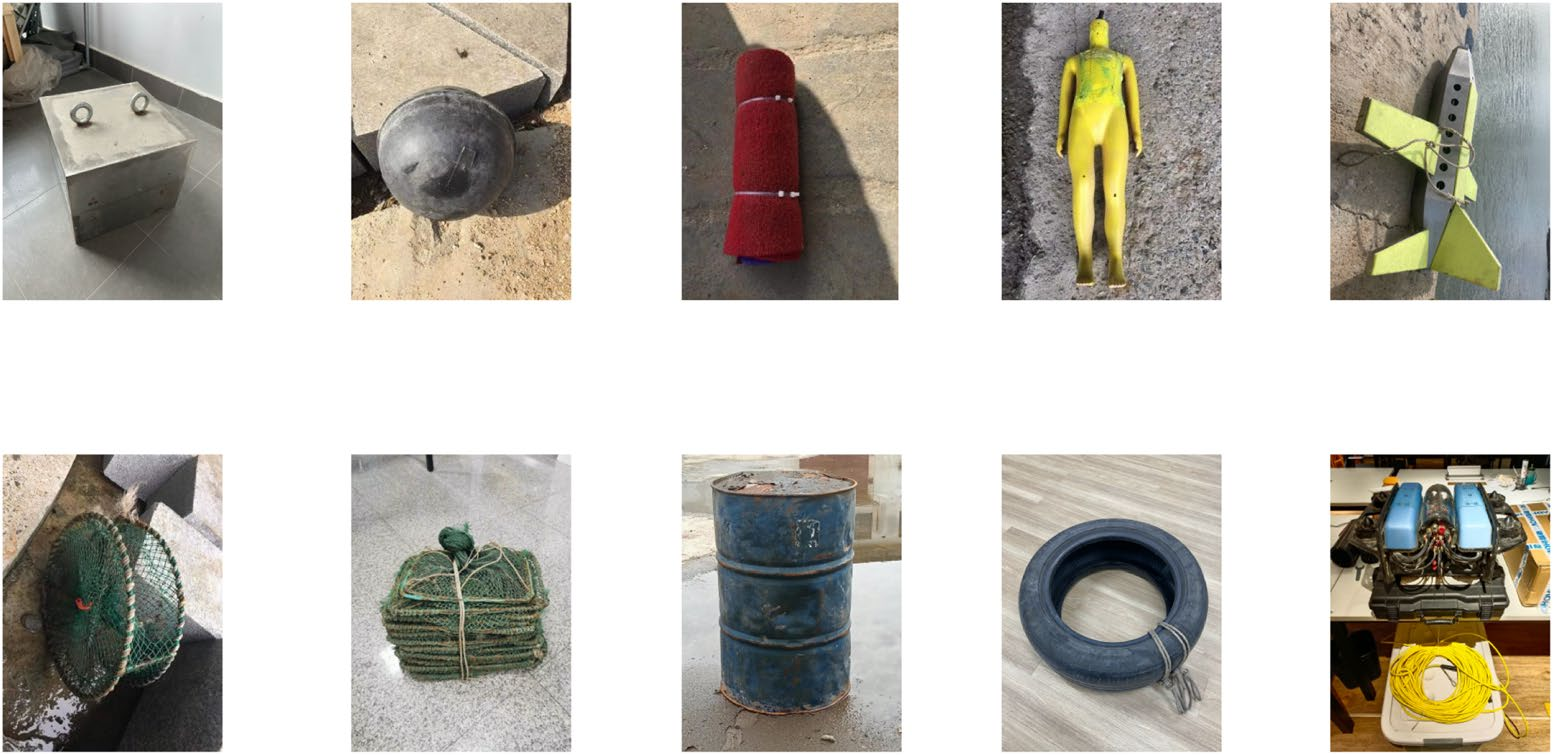
\includegraphics[width=\textwidth]{UATD_Objects.png}
    \caption[UATD Objecten.]{\label{fig:uatd_objects}Overzicht van objecten in de UATD-dataset. \autocite{Xie_2022}}
\end{figure}

De dataset wordt verspreid in een figshare-repository onder de CC BY 4.0 licentie. Deze licentie laat de gebruiker toe om het materiaal te delen en te bewerken, ook voor commerciële doeleinden. Buiten een naamsvermelding van de maker, een link naar de licentie en een vermelding of het werk al dan niet veranderd is, zijn er geen verdere restricties. De dataset wordt als ZIP-archief aangeboden. Gecomprimeerd is deze ongeveer 4,47 GB groot. Uitgepakt bevat ze drie aparte datasets en OpenSLT, de annotatietool die gebruikt werd, telkens opnieuw apart verpakt als ZIP-archief. De drie datasets zijn als volgt verdeeld: twee testsets -- \texttt{UATD\_Test\_1} en \texttt{UATD\_Test\_2} -- en één trainingsset -- \texttt{UATD\_Training}. Elk archief -- buiten die van de annotatietool natuurlijk -- bevat twee mappen: \texttt{annotations} en \texttt{images}. De map \texttt{annotations} bevat de annotaties en de map \texttt{images} bevat de sonarbeelden. \autocite{Jian_2022} \\

\begin{table}[H]
    \centering
    \begin{tabular}{llll}
        \toprule
        \textbf{Dataset} & \textbf{Aantal bestanden} & \textbf{Gecomprimeerde grootte} & \textbf{Ware grootte} \\
        \midrule
        UATD\_Test\_1  & 800  & 421.9 MB & 3.3 GB \\
        UATD\_Test\_2  & 800  & 424.6 MB & 3.3 GB \\
        UATD\_Training & 7600 & 3.9 GB   & 25.8 GB \\
        \bottomrule
    \end{tabular}
    \caption[Datasets binnen UATD]{\label{tab:uatd_datasets_overview} Tabel van eigenschappen van de datasets binnen de UATD-dataset. \autocite{Jian_2022}}
\end{table}

De bestanden volgen een vast benamingsschema zodat de beelden en de annotaties makkelijk aan elkaar gekoppeld kunnen worden. In elke dataset zijn de bestanden genummerd van \texttt{00001} tot aan het aantal bestanden in de dataset (bv. \texttt{00800} voor elke testset). Het beeld en de overeenkomstige annotatie hebben hetzelfde nummer. Zo zijn de paden voor het tweede beeld bijvoorbeeld:

\begin{itemize}
    \item \textbf{Beeld:} \texttt{UATD/UATD\_Test\_1/images/00003.bmp}
    \item \textbf{Annotatie:} \texttt{UATD/UATD\_Test\_1/annotations/00003.xml}
\end{itemize}

\begin{figure}[H]
    \centering
    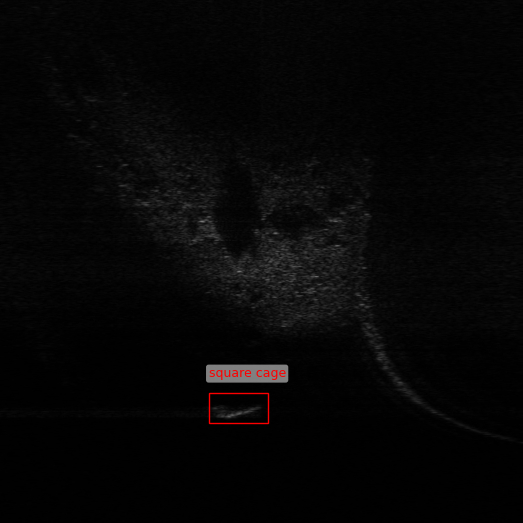
\includegraphics[width=0.5\textwidth]{UATD_example_annotated.png}
    \caption[UATD afbeelding met bounding boxes.]{\label{fig:uatd_image}Voorbeeld van een sonarbeeld binnen de UATD-dataset met de objecten aangeduid met \glspl{bounding_box} (afbeelding \texttt{UATD\_Test\_1/00003}). \autocite{Xie_2022}}
\end{figure}

De beelden zijn opgeslagen als 3-kanaals ongecomprimeerde BMP-bestanden met een bitdiepte van 8 bits (één byte). Dit is één van de eenvoudigste bestandsformaten om een foto op te slaan. Het bestand bevat namelijk een lijst van alle pixels, waarbij voor elke pixel het kleur wordt bijgehouden. Het kleur wordt in dit geval dus opgeslagen in 8 bits. Dit betekent dat het kleur van elke pixel bepaald wordt door een waarde tussen 0 en 255. Aangezien er drie kanalen zijn (RGB: Rood, Groen en Blauw), wordt elke pixel dus beschreven door $8 \times 3 = 24$ bits of 3 bytes. Als de afmetingen van de afbeelding gekend zijn, is het makkelijk om de grootte van de afbeelding te berekenen met behulp van volgende formule:

$$
\text{Grootte in Bytes} = \frac{breedte \times hoogte \times \#kanalen \times bitdiepte}{8}
$$ \\

Naast enkele tientallen bytes aan header- en fotodata is dit de werkelijke grootte van een BMP-bestand. Het nadeel is echter dat zo'n bestand heel snel heel groot wordt, aangezien BMP meestal gebruikt wordt zonder compressie. Anderzijds is zo'n verzameling van BMP-bestanden dan weer heel goed te comprimeren in bijvoorbeeld een ZIP-bestand. Zo kon de UATD-dataset van ongeveer 32,8 GB naar ongeveer 4,75 GB gecomprimeerd worden \footnote{Dit gaat over de som van de drie ZIP-bestanden die nog eens gezipt in de UATD-dataset zaten. De drie bestanden zijn dus nog eens gecomprimeerd, wat de grootte van het origineel gedownloade bestand op 4,47 GB bracht.}, wat op een compressiegraad van ongeveer 6.8 neerkomt. \autocite{Bourke_1998}

\begin{figure}[H]
    \centering
    \begin{tikzpicture}
        % Define parameters
        \def\imgSize{5}   % Image size (6x6 cm)
        \def\cellSize{1}  % Size of each cell
        \def\offset{7}    % Offset for second column
        \def\stackShift{0.5} % Shift for stacking channels
        \def\gridStep{\imgSize/5} % Step size for 6x6 grid
        
        % ==========================
        % First Column (Actual Image)
        % ==========================
        % Insert real image
        \node[anchor=south west, inner sep=0] (img) at (0,0) 
        {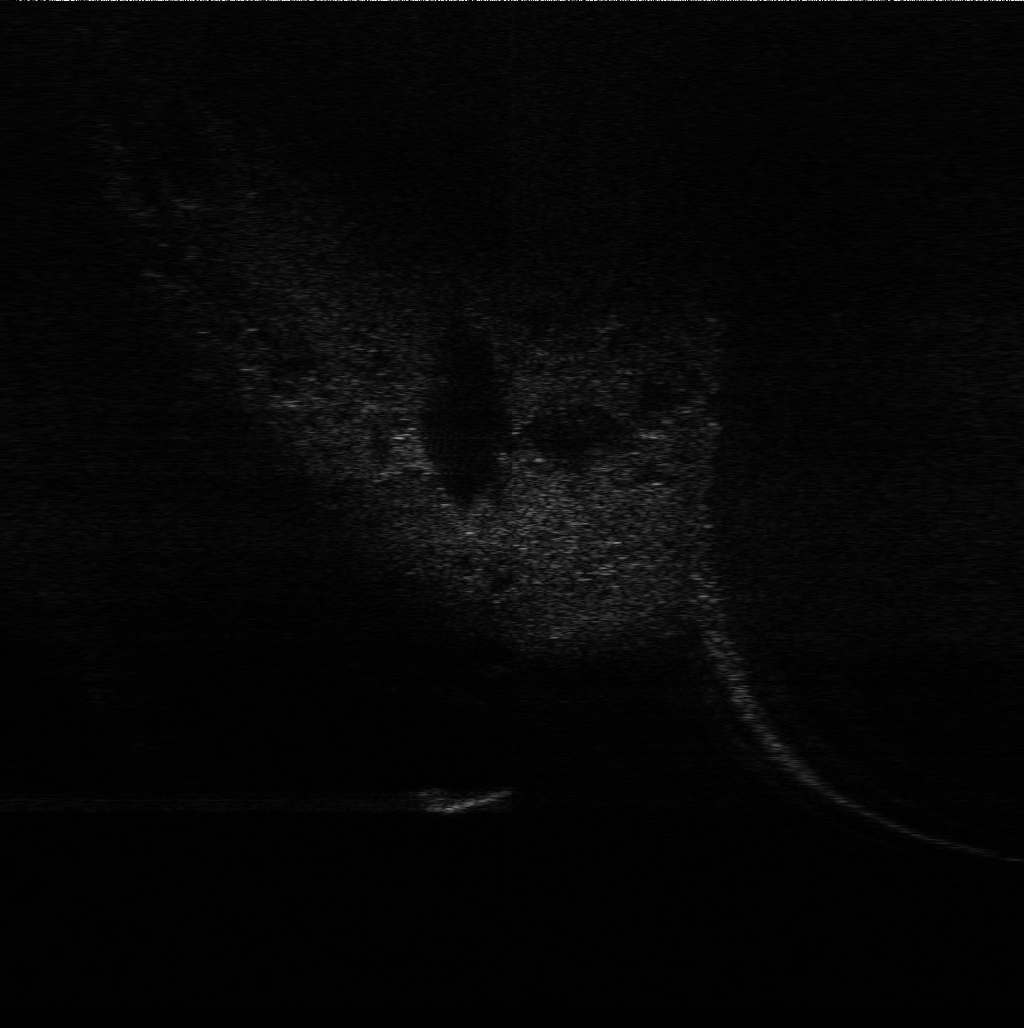
\includegraphics[width=\imgSize cm, height=\imgSize cm]{UATD_example.png}};
        
        % Draw white grid overlay (10x10)
        \draw[step=\gridStep,white, thick] (0,0) grid (\imgSize, \imgSize);
        
        % Image dimensions
        \draw[<->, thick] (-0.5, 0) -- (-0.5, \imgSize);
        \node[left] at (-0.5, \imgSize/2) {1028};
        
        \draw[<->, thick] (0, -0.5) -- (\imgSize, -0.5);
        \node[below] at (\imgSize/2, -0.5) {1024};
        
        % ==========================
        % Second Column (RGB Breakdown, Correct Stacking)
        % ==========================
        % 1. Blue Channel (furthest back, largest shift)
        \begin{scope}[shift={(\offset+2*\stackShift, 2*\stackShift)}]
            \fill[blue!50] (0,0) rectangle (\imgSize, \imgSize);
            \draw[white, thick, step=\gridStep] (0,0) grid (\imgSize, \imgSize);
        \end{scope}
        
        % 2. Green Channel (middle layer, medium shift)
        \begin{scope}[shift={(\offset+\stackShift, \stackShift)}]
            \fill[green!50] (0,0) rectangle (\imgSize, \imgSize);
            \draw[white, thick, step=\gridStep] (0,0) grid (\imgSize, \imgSize);
        \end{scope}
        
        % 3. Red Channel (front layer, no shift)
        \begin{scope}[shift={(\offset, 0)}]
            \fill[red!50] (0,0) rectangle (\imgSize, \imgSize);
            \draw[white, thick, step=\gridStep] (0,0) grid (\imgSize, \imgSize);
        \end{scope}
        
        % Dimensions for RGB squares
        \draw[<->, thick] (\offset-0.5, 0) -- (\offset-0.5, \imgSize);
        \node[left] at (\offset-0.5, \imgSize/2) {1028};
        
        \draw[<->, thick] (\offset, -0.5) -- (\offset+\imgSize, -0.5);
        \node[below] at (\offset+\imgSize/2, -0.5) {1024};
        
        % Diagonal arrow for number of channels (bottom-right corner)
        \draw[<->, thick] (\offset+0.7*\stackShift+\imgSize, -0.5) 
        -- (\offset+\stackShift+\imgSize+1, 0.5);
        \node[below] at (\offset+\stackShift+\imgSize+0.85, 0) {3};
        
    \end{tikzpicture}
    \caption[Voorbeeld van een bitmap.]{\label{fig:bitmap_example_image}Voorbeeld van de structuur van een bitmap-afbeelding zoals BMP.}
\end{figure}

Per afbeelding is er steeds een overeenkomstig XML-bestand dat de annotatie bevat. De annotatie volgt het Pascal \acrshort{voc}-formaat. Dit annotatieformaat werd origineel ontwikkeld voor de Visual Object Challenge. Deze challenge is een benchmark voor classificatie en objectdetectie die sinds 2005 jaarlijks georganiseerd wordt. Ondertussen is het formaat uitgegroeid tot een veelgebruikte standaard voor de annotatie van visuele datasets voor bijvoorbeeld objectdetectie. Door het gebruik van XML is het formaat makkelijk leesbaar. Echter maken heel weinig modellen rechtstreeks gebruik van het Pascal \acrshort{voc}-formaat, waardoor de annotatie meestal moet omgezet worden naar een ander formaat. \autocite{Everingham_2009}

\clearpage

\begin{listing}[H]
    \begin{minted}{xml}
        <annotation>
            <sonar>
                <range>24.9909</range>
                <azimuth>120</azimuth>
                <elevation>12</elevation>
                <soundspeed>1498.1</soundspeed>
                <frequency>1200k</frequency>
            </sonar>
            <file>
                <folder>UATD_Test_1</folder>
                <filename>00004</filename>
            </file>
            <size>
                <width>1024</width>
                <height>1257</height>
                <channel>3</channel>
            </size>
            <object>
                <name>rov</name>
                <bndbox>
                    <xmin>574</xmin>
                    <ymin>880</ymin>
                    <xmax>618</xmax>
                    <ymax>909</ymax>
                </bndbox>
            </object>
        </annotation>
    \end{minted}
    \caption[PASCAL VOC-annotatie]{Voorbeeld van een XML-bestand met annotatie voor objectdetectie in het PASCAL VOC-formaat (annotatie van \texttt{UATD\_Test\_1/00004}). \autocite{Xie_2022}}
\end{listing}

\subsubsection{SSS for Mine Detection}

Een andere mogelijke kandidaat is de \emph{\acrshort{sss} for Mine Detection}-dataset. Deze dataset bevat 1170 \emph{real-world} \gls{sss} sonarbeelden van de Portugese kust gemaakt door een gespecialiseerde \gls{auv}. Een dataset van deze grootte en kwaliteit verzamelen is geen sinecure, daarom is deze dataset verzameld in samenwerking met de Portugese marine. Specifiek werkten de onderzoekers gedurende verschillende jaren samen met \gls{dms3}. Dit team is verantwoordelijk voor alles wat met mijnen in zee te maken heeft. \autocite{Pessanha_Santos_2024}

\begin{figure}[H]
    \centering
    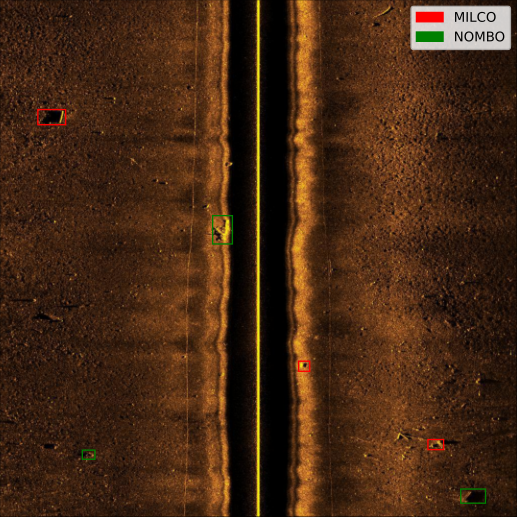
\includegraphics[width=0.5\textwidth]{SSSFMD_example_annotated.png}
    \caption[SSS for Mine Detection-afbeelding met bounding boxes.]{\label{fig:sssfmd_image}Voorbeeld van een sonarbeeld uit de \emph{\gls{sss} for Mine Detection}-dataset met de objecten aangeduid met \glspl{bounding_box} (afbeelding \texttt{SSS for Mine Detection/2015/0001\_2015}). \autocite{Pessanha_Santos_2024_SSSFMD}}
\end{figure}

Deze dataset is geschikt voor verschillende soorten ML-gerichte taken, waaronder objectdetectie, classificatie en segmentatie. De objecten in de dataset zijn geannoteerd met \glspl{bounding_box} om verschillende objecten aan te duiden. Deze vallen onder te verdelen in twee klassen: \glspl{milco} en \glspl{nombo}. Kortom: alles wat een mijn kan zijn en alles wat geen mijn kan zijn.

\begin{figure}[H]
    \centering
    \begin{tikzpicture}
        \begin{axis}[
            xbar stacked,
            width=\textwidth,
            height=0.45\textwidth,
            symbolic y coords={2010, 2015, 2017, 2018, 2021},
            ytick=data,
            xmin=0,
            xmax=450,
            bar width=15pt,
            enlarge y limits=0.3,
            legend style={at={(1,1)}, anchor=north east, legend columns=1},
            xlabel={Aantal objecten},
            ylabel={Jaar}
            ]
            % First column data (Bottom part of stacked bars)
            \addplot+[xbar, color=blue, fill=blue!50] coordinates {(12,2010) (175,2015) (2,2017) (46,2018) (0,2021)};
            \addlegendentry{\glspl{nombo}}
            
            % Second column data (Top part of stacked bars)
            \addplot+[xbar, color=red, fill=red!50] coordinates {(22,2010) (238,2015) (28,2017) (95,2018) (49,2021)};
            \addlegendentry{\glspl{milco}}
            
        \end{axis}
    \end{tikzpicture}
    \caption[Aantal objecten per jaar in SSS for Mine Detection.]{\label{fig:SSSFMD_objects_per_year}Grafiek van het aantal waargenomen objecten per jaar in de \emph{\gls{sss} for Mine Data}-dataset. \autocite{Pessanha_Santos_2024}}
\end{figure}

Ook deze dataset wordt verspreid in een figshare-repository onder de CC BY 4.0 licentie. Opnieuw wordt een ZIP-archief van ongeveer 584 MB aangeboden. Dit ZIP-archief bevat opnieuw andere ZIP's. Deze hebben de naam van één van de jaren waarvan er data beschikbaar is en bevatten dit dan ook. Daarnaast is er nog een ZIP-bestand met de gewichten van een getraind \gls{YOLO}v4-model en de code hiervoor. Dit is echter niet nuttig voor dit onderzoek en zal dus niet gebruikt worden. \\

In de mappen verdeeld per jaar zitten zowel de beelden als de annotaties (niet gescheiden). De beelden zijn JPG-bestanden. Het lijkt erop dat er twee verschillende resoluties gebruikt zijn voor de afbeeldingen, namelijk \texttt{416 x 416} en \texttt{1024 x 1024}. De afbeeldingen volgen een vast benamingsschema: elke afbeelding bevat een oplopend nummer beginnend van \texttt{0001}, daarna een underscore en dan het jaar waarin de afbeelding is gemaakt. Alles samen is dat dus bijvoorbeeld: \texttt{0001\_2015.jpg}. De bestanden met annotatie staan in dezelfde map en hebben dezelfde naam als hun overeenkomstige afbeeldingen. Het enige verschil is dat zij een \texttt{.txt}-extensie hebben. Dit tekstbestand bevat de annotatie in \gls{yolo}-formaat. \autocite{Pessanha_Santos_2024_SSSFMD}

\begin{listing}[H]
    \begin{minted}{text}
        0 0.10009765625 0.2265625 0.0537109375 0.029296875
        1 0.43017578125 0.4443359375 0.0380859375 0.0546875
        0 0.587890625 0.7080078125 0.021484375 0.01953125
        0 0.84228515625 0.859375 0.0302734375 0.01953125
        1 0.17138671875 0.87890625 0.0244140625 0.017578125
        1 0.91455078125 0.958984375 0.0478515625 0.02734375
    \end{minted}
    \caption[YOLO-annotatie]{Voorbeeld van een TXT-bestand met annotatie voor objectdetectie in het YOLO-formaat (annotatie van \texttt{SSS for Mine Detection/2015/0001\_2015}). \autocite{Pessanha_Santos_2024_SSSFMD}}
\end{listing}

Eigenlijk is dit niks meer dan een CSV-bestand waarbij de separator een spatie is. In getabelleerde vorm is de data iets overzichtelijker.

\begin{table}[H]
    \centering
    \begin{tabular}{lllll}
        \toprule
        \textbf{Klasse} & \textbf{$x$-coördinaat} & \textbf{$y$-coördinaat} & \textbf{Hoogte} & \textbf{Breedte} \\
        \midrule
        0 & 0.10009765625 & 0.2265625    & 0.0537109375 & 0.029296875 \\
        1 & 0.43017578125 & 0.4443359375 & 0.0380859375 & 0.0546875   \\
        0 & 0.587890625   & 0.7080078125 & 0.021484375  & 0.01953125  \\
        0 & 0.84228515625 & 0.859375     & 0.0302734375 & 0.01953125  \\
        1 & 0.17138671875 & 0.87890625   & 0.0244140625 & 0.017578125 \\
        1 & 0.91455078125 & 0.958984375  & 0.0478515625 & 0.02734375  \\
        \bottomrule
    \end{tabular}
    \caption[YOLO-annotatie in getabelleerde vorm]{\label{tab:yolo_annot_table} Tabel met annotatie voor objectdetectie in het YOLO-formaat (annotatie van \texttt{SSS for Mine Detection/2015/0001\_2015}). \autocite{Pessanha_Santos_2024_SSSFMD}}
\end{table}

Merk op dat de klasse \texttt{0} of \texttt{1} is. Uit de paper van \textcite{Pessanha_Santos_2024} blijkt dat \texttt{0} een \gls{milco} is en \texttt{1} een \gls{nombo}. De volgende vier kolommen stellen een \gls{bounding_box} voor. Er bestaan verschillende formaten om zo'n \gls{bounding_box} voor te stellen. Dit formaat gebruikt één coördinaat ($(x, y)$) die het midden van de \gls{bounding_box} voorstelt, de hoogte en de breedte. \\

Men zou verwachten dat deze waarden gegeven zijn in pixels. Dat brengt echter een probleem met zich mee wanneer de afbeelding geschaald wordt. Dan moeten de pixelwaarden telkens herberekent worden om zo de \gls{bounding_box} op de juiste plaats op de afbeelding te laten vallen. Om dit op te lossen worden deze waarden -- zoals hier -- meestal als verhoudingen uitgedrukt. Zo is de breedte bijvoorbeeld de breedte in pixels gedeeld door de breedte van de afbeelding.

\begin{figure}[H]
    \centering
    \begin{tikzpicture}
        
        % Draw the outer rectangle (image)
        \draw[thick] (0,0) rectangle (7,7);
        % Label the dimensions of the outer rectangle
        \draw[<->] (-0.5,0) -- (-0.5,7) node[midway, left] {$h_{image}$};
        \draw[<->] (0,-0.5) -- (7,-0.5) node[midway, below] {$w_{image}$};
        
        % Draw the bounding box inside the image
        \draw[thick, dashed] (2,2) rectangle (5,5);
        % Label the dimensions of the bounding box
        \draw[<->] (1.5,2) -- (1.5,5) node[midway, left] {$h_{bb}$};
        \draw[<->] (2,1.5) -- (5,1.5) node[midway, below] {$w_{bb}$};
        
        % Add a dot in the center of the bounding box
        \filldraw [black] (3.5,3.5) circle (2pt);
        % Label the coordinates of the dot
        \node at (3.5,3) {$(x_{bb}, y_{bb})$};
        
    \end{tikzpicture}
    \caption[Structuur van een bounding box.]{\label{fig:bounding_box}Structuur van een \gls{bounding_box} (gebaseerd op een figuur van \textcite{Pessanha_Santos_2024})}.
\end{figure}

Als de afbeelding geschaald wordt, schaalt de \gls{bounding_box} mee en kan men aan de hand van een relatief eenvoudige formule terug de pixelwaarde berekenen zonder complexe transformaties op de \gls{bounding_box} te moeten gaan toepassen. De formule om de absolute pixelwaarden om te zetten naar relatieve verhoudingen is de volgende:

$$
(x,y,w,h) = \left(\frac{x_{bb}}{w_{image}},\frac{y_{bb}}{h_{image}},\frac{w_{bb}}{w_{image}},\frac{h_{bb}}{h_{image}}\right)
$$ 

\clearpage

Naast het verzamelen van de dataset trainden de onderzoekers ook een objectdetectiemodel -- namelijk \gls{yolo}v4 -- op deze data om de kwaliteit ervan te testen. De configuratie voor het trainingsproces werd speciaal aangepast om de performance van dit model te verhogen. De \gls{batch_size} werd ingesteld op 64 en werden gedurende de training opgesplitst in 16 \glspl{mini_batch} van elk 4 afbeeldingen, dit om het geheugengebruik tijdens het trainingsproces te optimaliseren. \\

Het maximum aantal \glspl{batch} werd ingesteld op 6000. Ook werd de \gls{learning_rate} van het model op kritieke punten aangepast, namelijk na het verwerken van 4800 en 5400 \glspl{batch}, dit om de convergentie te verhogen. Ook pasten de onderzoekers transfer learning toe door de gewichten van het model te initialiseren met gewichten van de \gls{coco}-dataset. Na het model te trainen op de volledige dataset van 1170 afbeeldingen, behaalde deze een \gls{iou} van 60\% en een \gls{map} van 75\%. Ook werd een \gls{precision} van 82\% en een \gls{recall} van 64\% behaald. \autocite{Pessanha_Santos_2024}

\subsubsection{UXO}

Ten slotte is er de \acrshort{uxo}-dataset. \acrshort{uxo} is de afkorting voor \acrlong{uxo}, de Engelse benaming voor \glspl{blindganger}. Dit is meteen ook de inhoud van deze dataset. Ze bevat namelijk 74 437 afbeeldingen van \glspl{blindganger} en is daarmee de grootste dataset die in dit onderzoek voorkomt. Het doel van deze dataset is om een validatieset te zijn en ze is samengesteld om onderzoek naar ontmijning in plassen, meren, zeeën en oceanen vooruit te helpen. Zoals al eerder vermeld is dit onderwerp zeer gevoelig en wordt er meestal (lees: bijna altijd) voor gekozen om deze datasets zo confidentieel mogelijk te houden. Daarom bevat deze dataset ook geen \emph{real-world}-afbeeldingen. In plaats daarvan zijn beelden in een gecontroleerde, experimentele omgeving gemaakt. \autocite{Dahn_2024_UXO}

\begin{figure}[H]
    \centering
    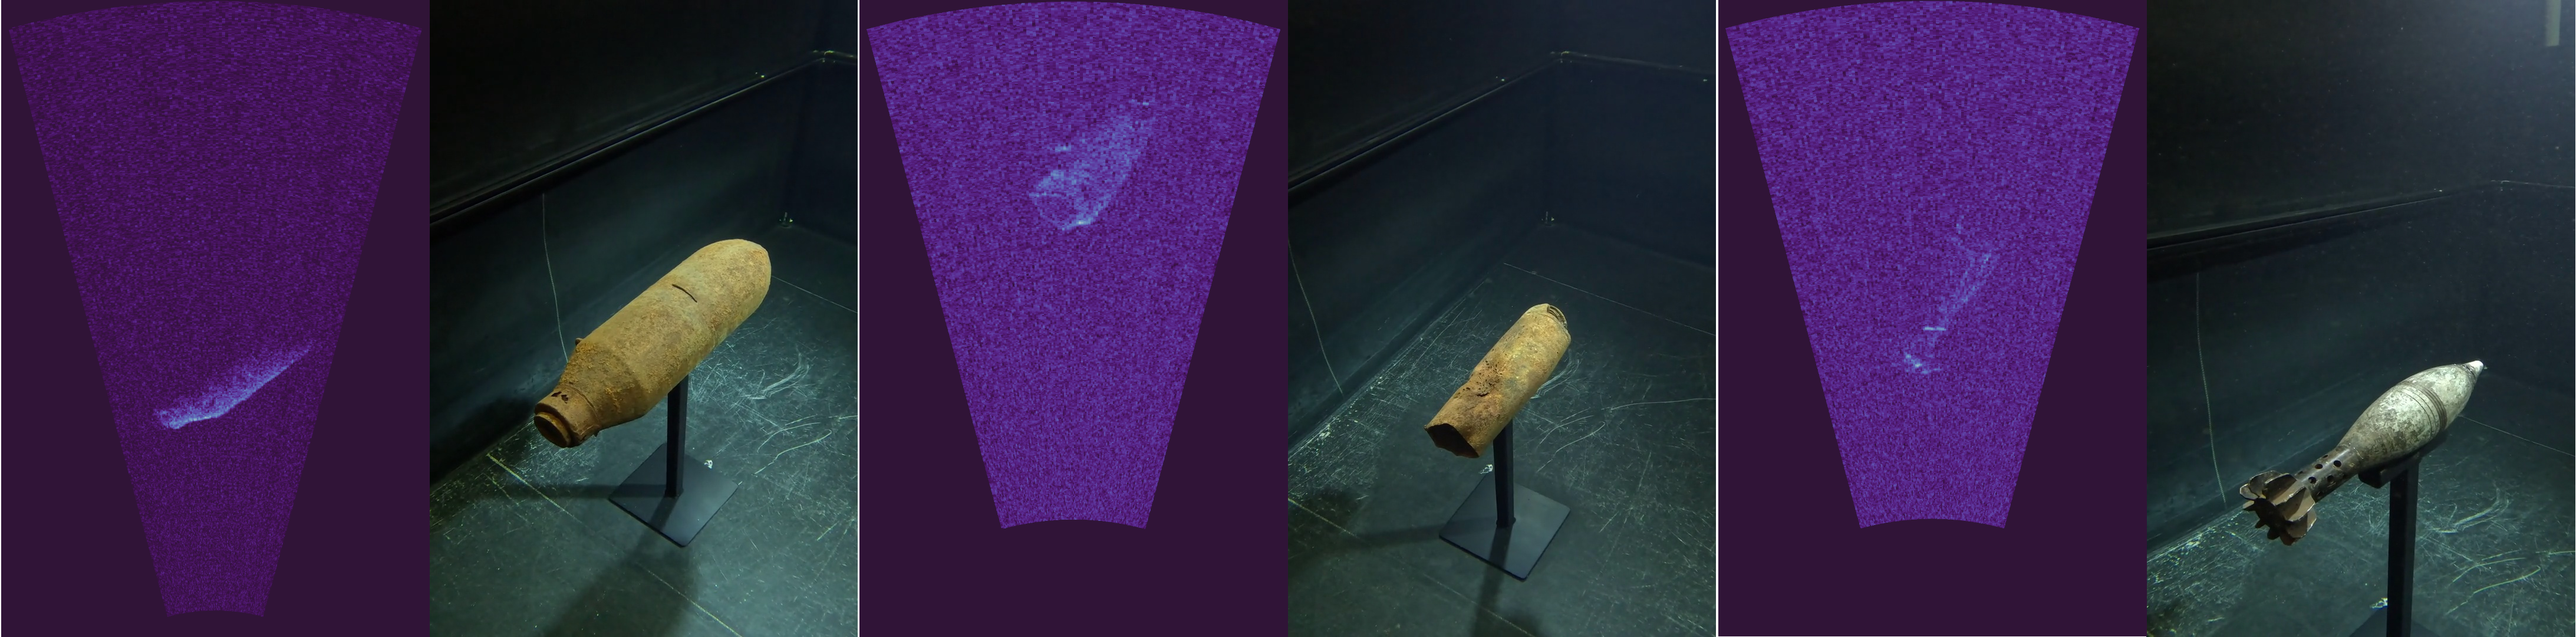
\includegraphics[width=\textwidth]{teaser_uxo.png}
    \caption[Voorbeeld van sonarbeelden \& afbeeldingen in de UXO-dataset]{\label{fig:uxo_teaser}. Voorbeeld van sonarbeelden en overeenkomstige afbeeldingen van verschillende type \glspl{blindganger} in de UXO-dataset. \autocite{Dahn_2024_UXO}}
\end{figure}

Om deze dataset samen te stellen, hebben de onderzoekers een volledig gecontroleerde testopstelling gemaakt bij het \gls{dfki}, het Duits onderzoekscentrum voor artificiële intelligentie in Bremen. De dataset is gemaakt met een ARIS Explorer 3000 sonarmodule (voor de sonarbeelden) en een GoPro Hero 8 (voor de bijhorende 5,3K UHD afbeeldingen). Deze twee modules werden op een \gls{PTU} (de ARIS Rotator AR3) gemonteerd die vastzat aan een op maat gemaakte \gls{portaalkraan}. Deze kraan kon vrij in de $xyz$-assen bewegen en kon verschillende voorgeprogrammeerde banen heel precies volgen. 

\begin{figure}[H]
    \centering
    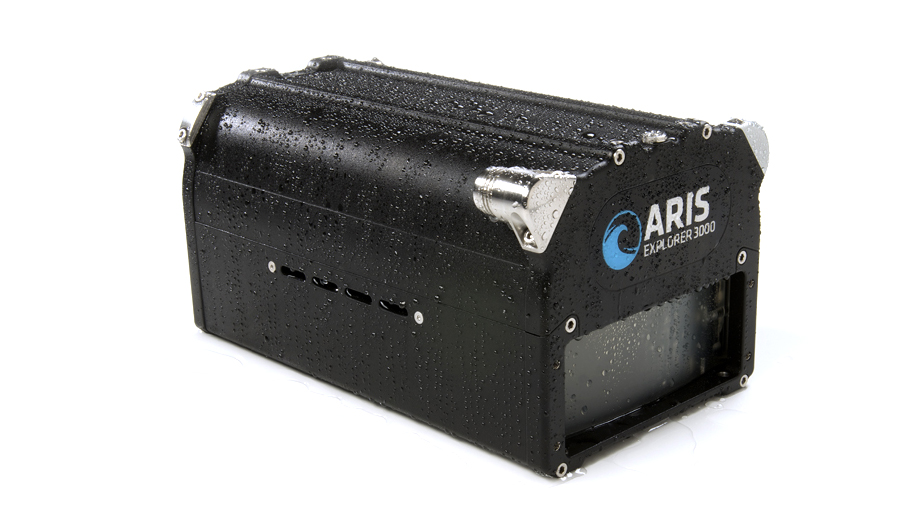
\includegraphics[width=0.5\textwidth]{ARIS-3000.jpg}
    \caption[Afbeelding van de ARIS Explorer 3000]{\label{fig:aris_3000}. Afbeelding van de ARIS Explorer 3000 sonarmodule. \autocite{soundmetrics.com}}
\end{figure}

Om de omgeving van de zee zo goed mogelijk te kunnen nabootsen, bouwden de onderzoekers een bassin gevuld met 20 000 liter zoetwater. Hierin plaatsten ze verschillende \emph{targets}, de \glspl{blindganger}. Deze waren aangeleverd door EGGERS Kampfmittelbergung GmbH, een bedrijf dat zich bezighoudt met het ontmijnen van verschillende sites. Om de veiligheid te garanderen, werden de \glspl{blindganger} voordien onschadelijk gemaakt. Er werden verschillende \glspl{blindganger} gebruikt om zo variëteit in de dataset te garanderen: een normale bom van ongeveer 51 kg, een vervormde fosforbom en een mortier. \autocite{Dahn_2024}

\begin{figure}[H]
    \centering
    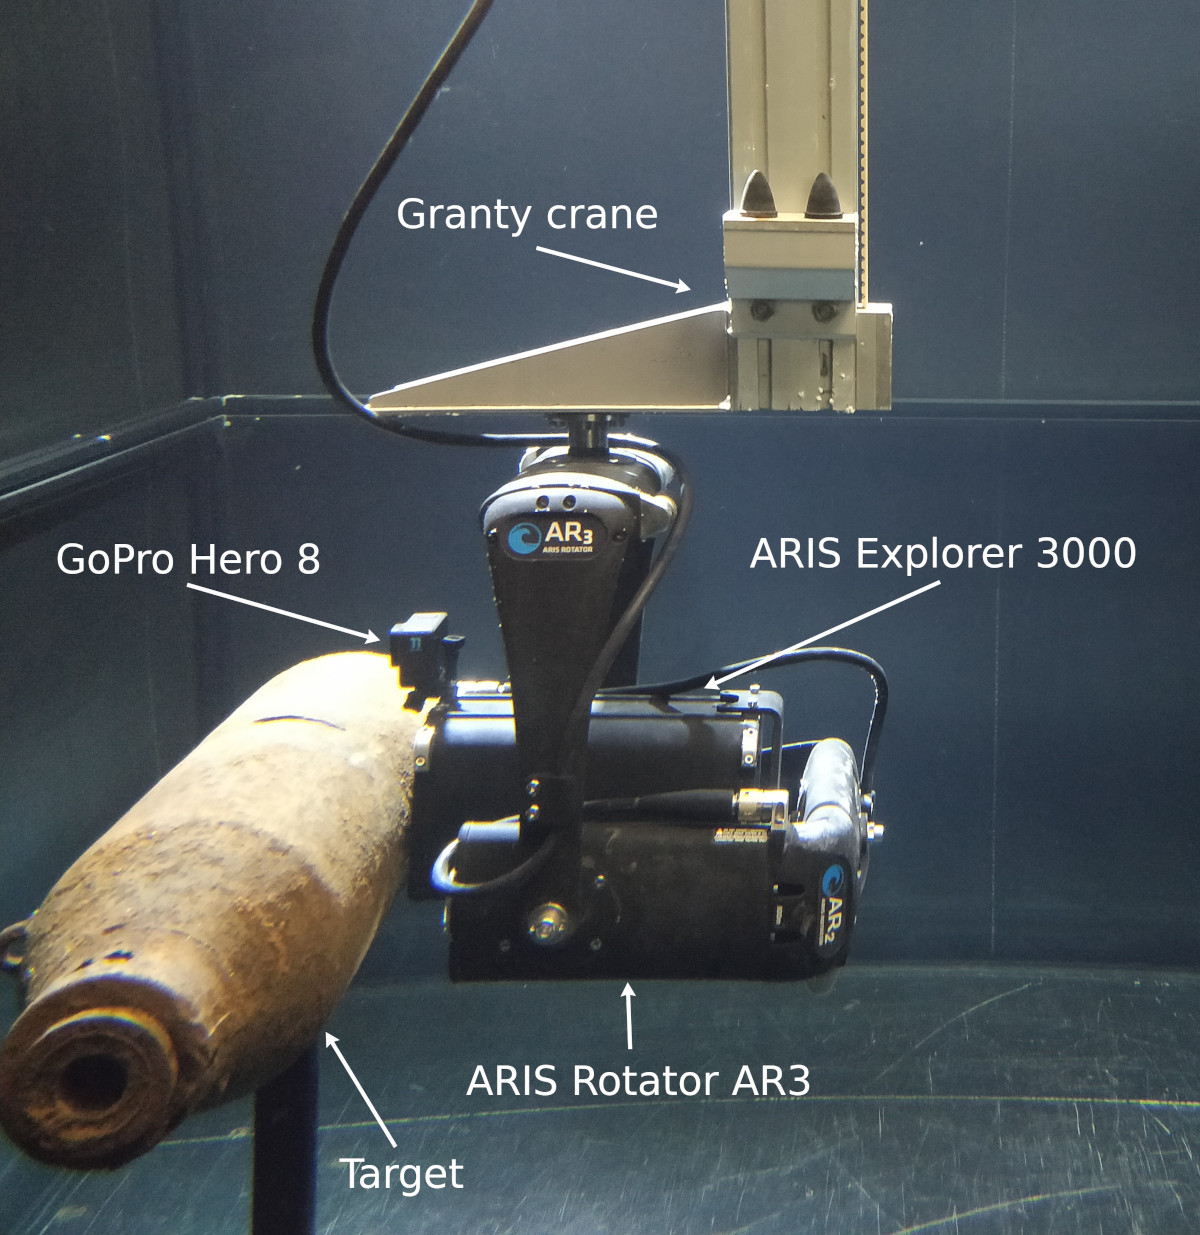
\includegraphics[width=0.5\textwidth]{uxo_setup.jpg}
    \caption[Setup waarmee de UXO-dataset gemaakt is]{\label{fig:uxo_setup}. Afbeelding van de setup die gebruikt werd om data te verzamelen voor de UXO-dataset. \autocite{Dahn_2024_UXO}}
\end{figure}

De dataset is alles samen zo'n 94,7 GB groot. Ze is de meest uitgebreide die in dit onderzoek voorkomt, niet alleen qua grootte, maar ook qua inhoud. De dataset is onderverdeeld in verschillende mappen. De map \texttt{3d\_models} bevat 3D-modellen van de \glspl{blindganger}. De map \texttt{calibration} bevat dan weer de transformaties tussen de kraan en de sensors en de kalibraties van de GoPro. Het merendeel van de dataset zit in de map \texttt{recordings}. Deze bevat mappen per type \gls{blindganger}. In deze mappen zitten dan telkens weer mappen met de datum en tijd van elk experiment. Deze mappen bevatten verschillende mappen en bestanden die de \emph{core} van de data vormen. \autocite{Dahn_2024_UXO}

\clearpage

\begin{itemize}
    \item \textbf{\texttt{aris\_raw}:} map die de \emph{raw} sonarbeelden bevat in PGM formaat. Dit is een eenvoudig rasterafbeeldingsformaat (zoals BMP, cf. figuur \ref{fig:bitmap_example_image}) dat grijswaardenafbeeldingen opslaat. PGM-bestanden kunnen in een ASCII (tekst) of binaire (snellere) variant worden opgeslagen. Elke pixel heeft een intensiteitswaarde tussen 0 (zwart) en een maximumwaarde (meestal 255, wit), waardoor verschillende grijstinten mogelijk zijn. De afbeelding bevat ook een header met het formaat, afmetingen en maximale intensiteit, gevolgd door de pixelgegevens. PGM wordt vaak gebruikt in beeldverwerking en wetenschappelijke toepassingen vanwege de eenvoud en brede compatibiliteit. \autocite{Poskanzer_2016}
    \item \textbf{\texttt{aris\_polar}:} map die de poolgetransformeerde sonarbeelden bevat in PNG formaat.
    \item \textbf{\texttt{gopro}:} map die de beelden in JPG formaat bevat die gemaakt zijn door de GoPro.
    \item \textbf{\texttt{labels}:} map die annotatie van \glspl{bounding_box} bevat in JSON formaat.
    \item \textbf{\texttt{aris\_file\_meta.yaml}:} YAML-bestand met de metadata van de sonar 
    \item \textbf{\texttt{aris\_frame\_meta.csv}:} CSV-bestand met metadata voor elk sonarframe, inclusief \gls{ptu}-informatie.
    \item \textbf{\texttt{gantry.csv}:} CSV-bestand met posities van de \gls{portaalkraan} bij elk sonarframe.
    \item \textbf{\texttt{notes.txt}:} TXT-bestand met korte beschrijving over experiment.
\end{itemize}

\begin{figure}[H]
    \centering
    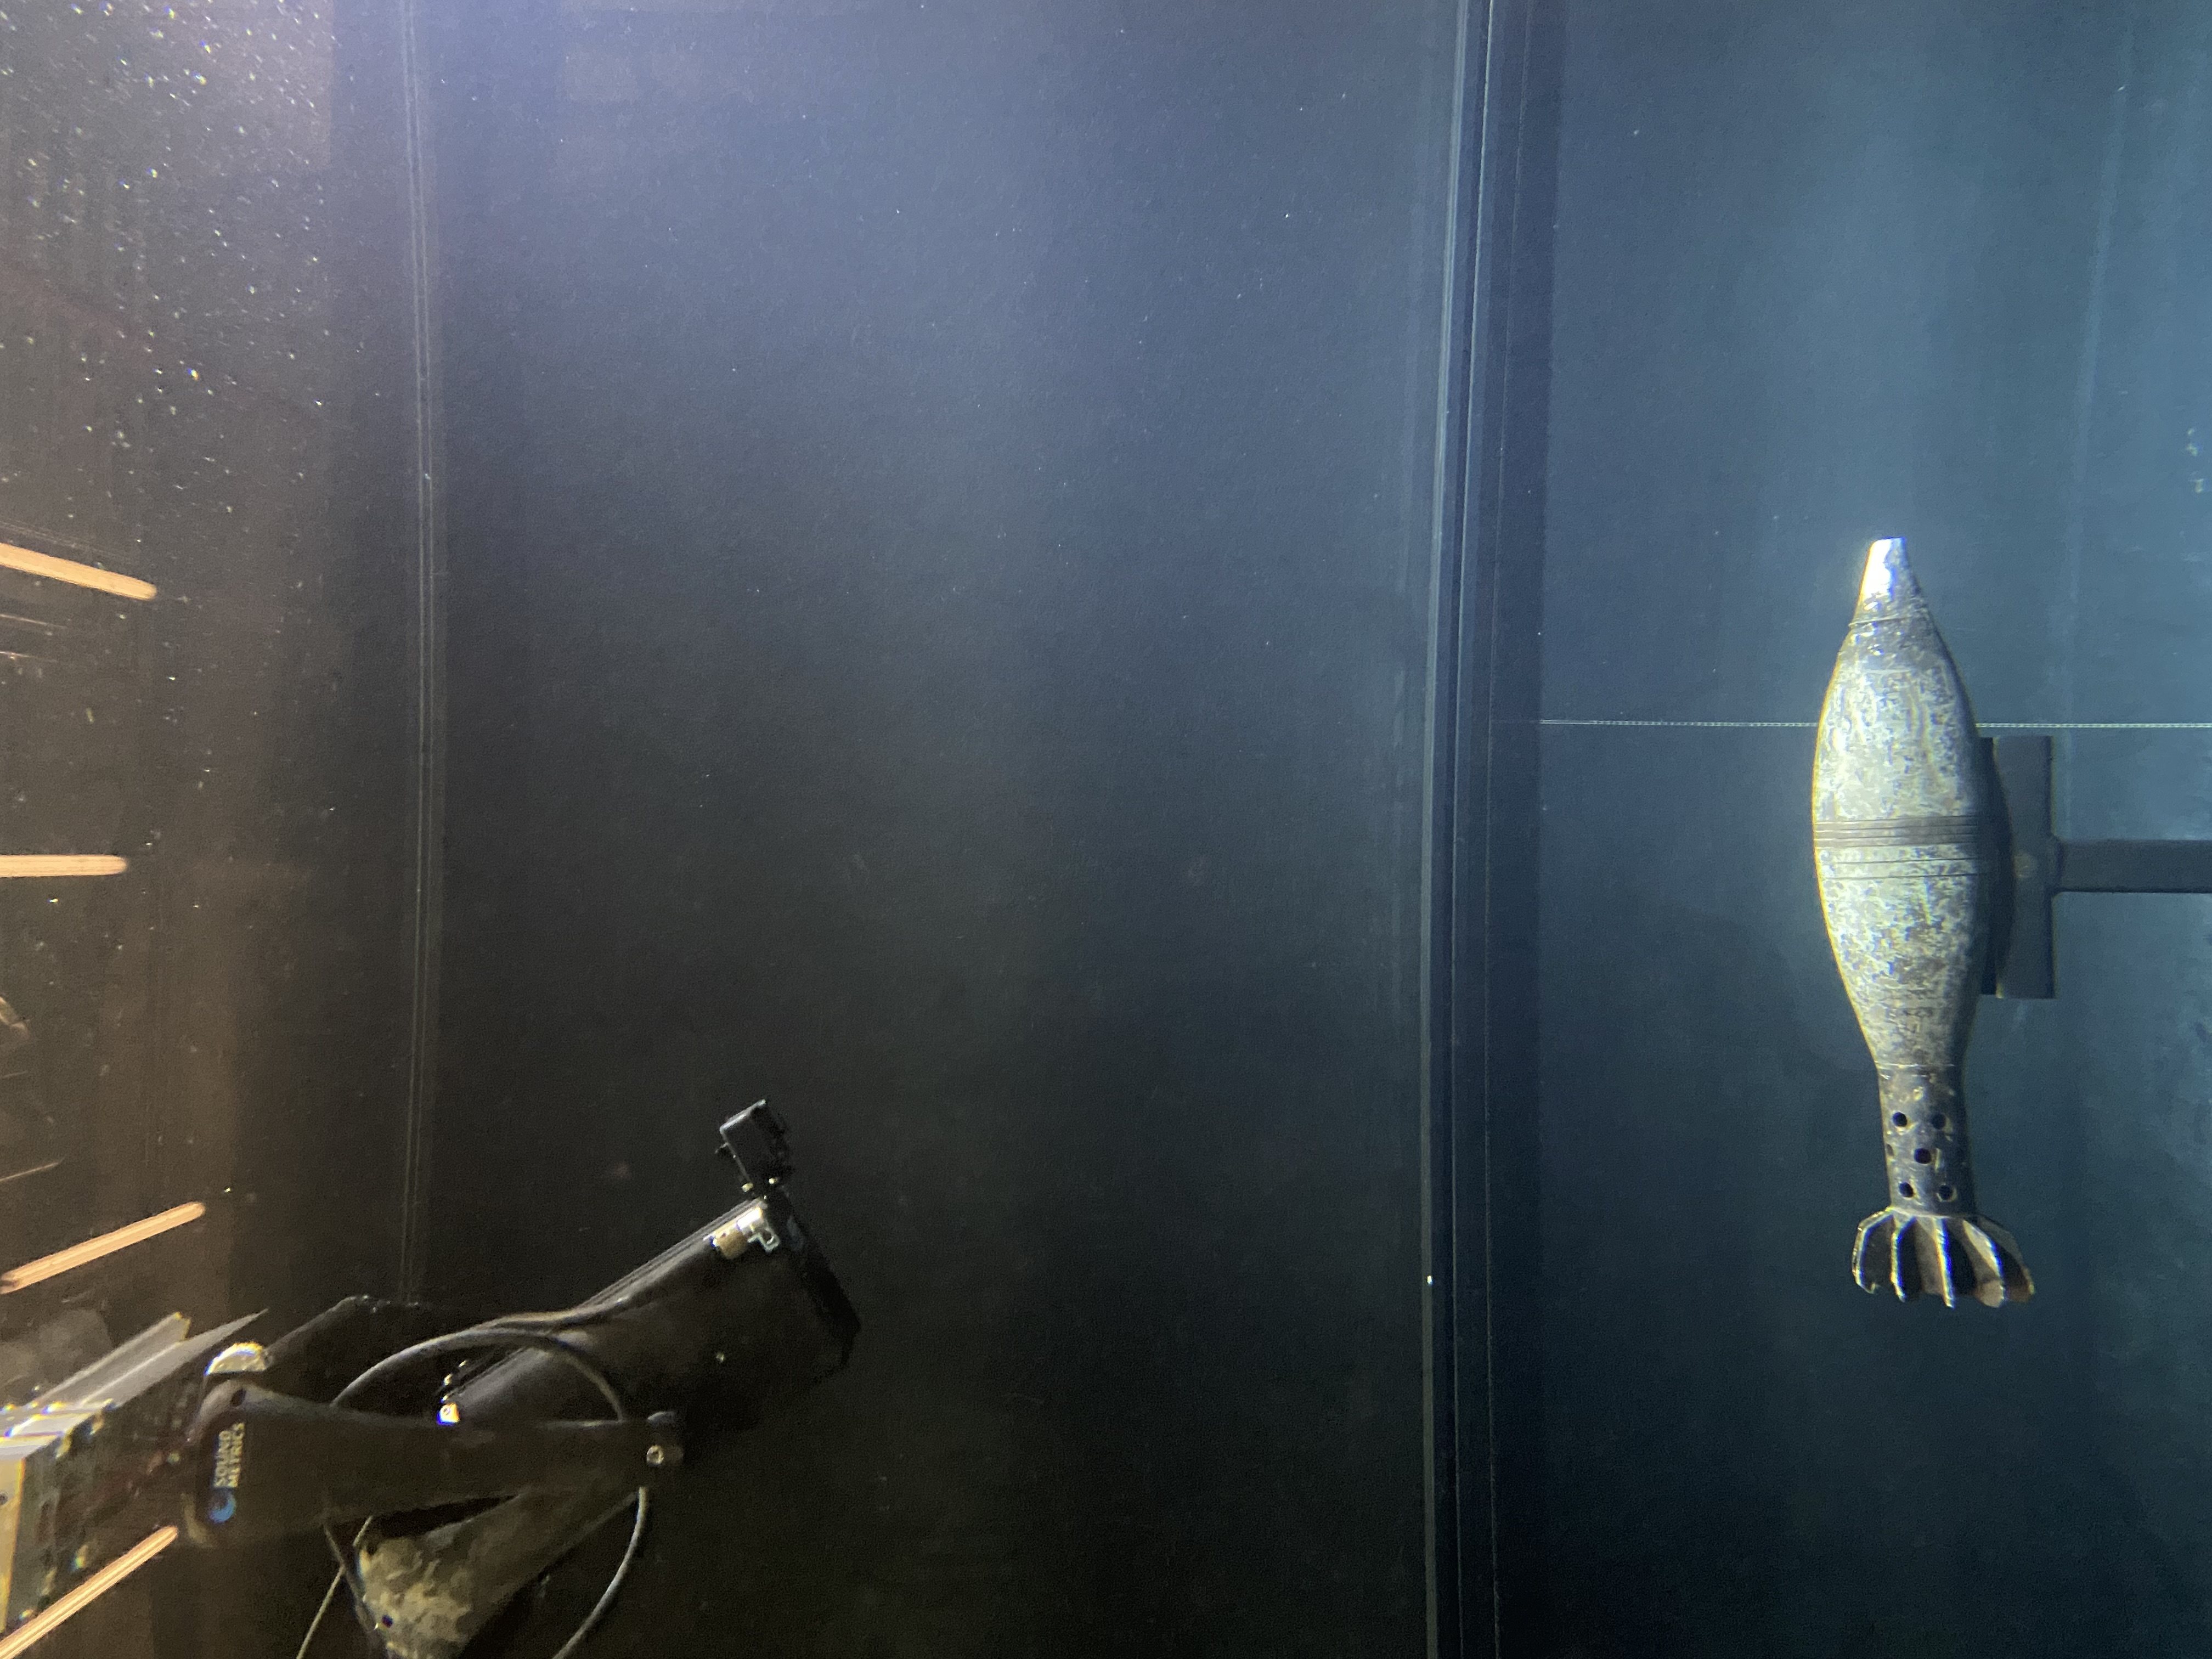
\includegraphics[width=0.5\textwidth]{uxo_preview.jpg}
    \caption[UXO-setup in actie]{\label{fig:uxo_preview}. Preview van de setup waarmee de UXO-dataset is gemaakt in actie. \autocite{Dahn_2024_UXO}}
\end{figure}

\clearpage

\subsubsection{Conclusie}

Alle drie de datasets die hierboven besproken werden, maken het mogelijk om een objectdetectiemodel mee te trainen. Ze bieden namelijk allemaal annotaties van \glspl{bounding_box} op de bijhorende afbeeldingen aan. Daarnaast zijn deze datasets makkelijk te verwerken, aangezien alle beelden in conventionele afbeeldingsformaten zijn opgeslagen (zoals PNG, JPG, BMP, PGM, \dots). Toch is er -- specifiek voor dit onderzoek -- één dataset die geschikter is dan de anderen. De UATD-dataset is -- misschien ietwat subjectief -- uitgekozen om te gebruiken in de rest van dit onderzoek. Dit komt omdat ze bepaalde aspecten aanbiedt die de andere datasets niet hebben. \\

\gls{sss} for Mine Detection lijkt op het eerste zicht de perfecte dataset voor dit onderzoek. Het probleem is echter dat ze relatief klein is: ze bevat ``slechts'' 1170 afbeeldingen. Op het eerste zicht lijkt dit voldoende. Echter moet deze dataset nog opgesplitst worden in -- ten minste -- een trainingsset en een testset.\footnote{In een optimale situatie zou de data opgesplitst worden in drie sets: een trainingsset, een testset en een validatieset. Dit komt omdat de validatiedataset -- hoewel ze niet gebruikt wordt om het model te trainen -- gebruikt wordt om de paramaters van het model te tunen. Dit kan leiden tot \gls{overfitting}. Het is beter om als testset data te gebruiken dat het model nog niet gezien heeft. \autocite{Goodfellow_2016}} Ook komen er slechts 668 objecten voor in de dataset. Tot overmaat van ramp zijn deze ook zeer slecht verdeeld. 

\begin{table}[H]
    \centering
    \begin{tabular}{ll}
        \toprule
        \textbf{\# objecten / beeld} & \textbf{\# beelden} \\
        \midrule
        13 & 1 \\
        9  & 2 \\
        8  & 4 \\
        7  & 8 \\
        6  & 8 \\
        5  & 13 \\
        4  & 9 \\
        3  & 41 \\
        2  & 59 \\
        1  & 159 \\
        0  & 866 \\
        \bottomrule
    \end{tabular}
    \caption[Aantal objecten per afbeelding in SSS for Mine Data]{\label{tab:objects_per_image_sss} Tabel met verdeling van objecten per afbeelding in de \gls{sss} for Mine Detection-dataset.}
\end{table}

\clearpage

Er is één afbeelding met wel 13 objecten en 866 zonder ook maar één object. Door deze slechte verdeling en de beperkte hoeveelheid data in de dataset is ze dus weinig bruikbaar voor dit onderzoek. \\

Dit is een probleem waar de UXO-dataset absoluut niet mee kampt. Deze heeft dan echter weer andere problemen. De dataset is namelijk volledig samengesteld in een gecontroleerde testopstelling. Ze bevat dus geen \emph{real-world}-data. Dit betekent echter ook dat bepaalde artefacten en afwijkingen typisch aan meren en zeeën niet in deze dataset voorkomen. De beelden zijn zodanig zuiver dat het hoogstwaarschijnlijk mogelijk zou zijn om de \glspl{blindganger} te herkennen door te zoeken naar de groep helderste pixels of met een edge-detection algoritme. \autocite{Torre_1986} \\

Ook de grootte van de dataset is misschien iets te mooi om waar te zijn. De beelden in de dataset zijn namelijk geen onafhankelijke afbeeldingen, maar frames van een continue opname. Dit zorgt ervoor dat er (nagenoeg) geen verschil is tussen afbeelding $n$ en afbeelding $n+1$. Als alle afbeeldingen na elkaar worden afgespeeld, ziet men een opname van een transformatie (rotatie, verschuiving, \dots) van één van de \glspl{blindganger}. Ten slotte staat er telkens maar één object op een afbeelding, wat multiple objectdetectie (meerdere objecten op één afbeelding herkennen) onmogelijk maakt.
%%=============================================================================
%% Methodologie
%%=============================================================================

\chapter{Methodologie}%
\label{ch:methodologie}

Dit onderzoek volgt een gestructureerde aanpak om semi- en self-supervised learning technieken voor objectdetectie in sonardata te implementeren en te evalueren. In deze methodologie wordt een onderverdeling gemaakt van de verschillende fasen in dit onderzoek. Hierbij wordt de basis gelegd voor de experimenten die zullen worden uitgevoerd in de proof of concept.

\section{Data-acquisitie}

Allereerst moet er een keuze gemaakt worden voor het gebruik van een dataset in het verdere verloop van dit onderzoek. Alle drie de datasets die in \ref{subsec:mogelijke-oplossingen} besproken werden, maken het mogelijk om een objectdetectiemodel mee te trainen. Ze bieden namelijk allemaal annotaties van \glspl{bounding_box} op de bijhorende afbeeldingen aan. Daarnaast zijn deze datasets makkelijk te verwerken, aangezien alle beelden in conventionele afbeeldingsformaten zijn opgeslagen (zoals PNG, JPG, BMP, PGM, \dots). Toch is er -- specifiek voor dit onderzoek -- één dataset die geschikter is dan de anderen. De UATD-dataset is -- misschien ietwat subjectief -- uitgekozen om te gebruiken in de rest van dit onderzoek. Dit komt omdat ze bepaalde aspecten aanbiedt die de andere datasets niet hebben. \\

\gls{sss} for Mine Detection lijkt op het eerste zicht de perfecte dataset voor dit onderzoek. Het probleem is echter dat ze relatief klein is: ze bevat ``slechts'' 1170 afbeeldingen. Op het eerste zicht lijkt dit voldoende. Echter moet deze dataset nog opgesplitst worden in -- ten minste -- een trainingsset en een testset.\footnote{In een optimale situatie zou de data opgesplitst worden in drie sets: een trainingsset, een testset en een validatieset. Dit komt omdat de validatiedataset -- hoewel ze niet gebruikt wordt om het model te trainen -- gebruikt wordt om de paramaters van het model te tunen. Dit kan leiden tot \gls{overfitting}. Het is beter om als testset data te gebruiken dat het model nog niet gezien heeft. \autocite{Goodfellow_2016}} Ook komen er slechts 668 objecten voor in de dataset. Tot overmaat van ramp zijn deze ook zeer slecht verdeeld. 

\begin{table}[H]
    \centering
    \begin{tabular}{ll}
        \toprule
        \textbf{\# objecten / beeld} & \textbf{\# beelden} \\
        \midrule
        13 & 1 \\
        9  & 2 \\
        8  & 4 \\
        7  & 8 \\
        6  & 8 \\
        5  & 13 \\
        4  & 9 \\
        3  & 41 \\
        2  & 59 \\
        1  & 159 \\
        0  & 866 \\
        \bottomrule
    \end{tabular}
    \caption[Aantal objecten per afbeelding in SSS for Mine Data]{\label{tab:objects_per_image_sss} Tabel met verdeling van objecten per afbeelding in de \gls{sss} for Mine Detection-dataset.}
\end{table}

Er is één afbeelding met wel 13 objecten en 866 zonder ook maar één object. Door deze slechte verdeling en de beperkte hoeveelheid data in de dataset is ze dus weinig bruikbaar voor dit onderzoek. \\

Dit is een probleem waar de UXO-dataset absoluut niet mee kampt. Deze heeft dan echter weer andere problemen. De dataset is namelijk volledig samengesteld in een gecontroleerde testopstelling. Ze bevat dus geen \emph{real-world}-data. Dit betekent echter ook dat bepaalde artefacten en afwijkingen typisch aan meren en zeeën niet in deze dataset voorkomen. De beelden zijn zodanig zuiver dat het hoogstwaarschijnlijk mogelijk zou zijn om de \glspl{blindganger} te herkennen door te zoeken naar de groep helderste pixels of met een edge-detection algoritme. \autocite{Torre_1986} \\

Ook de grootte van de dataset is misschien iets te mooi om waar te zijn. De beelden in de dataset zijn namelijk geen onafhankelijke afbeeldingen, maar frames van een continue opname. Dit zorgt ervoor dat er (nagenoeg) geen verschil is tussen afbeelding $n$ en afbeelding $n+1$. Als alle afbeeldingen na elkaar worden afgespeeld, ziet men een opname van een transformatie (rotatie, verschuiving, \dots) van één van de \glspl{blindganger}. Ten slotte staat er telkens maar één object op een afbeelding, wat multiple objectdetectie (meerdere objecten op één afbeelding herkennen) onmogelijk maakt.

\section{Dataverdeling}

In dit onderzoek zullen verschillende modellen getraind worden met verschillende leertechnieken. Daarom is het belangrijk om een duidelijk zicht te krijgen op hoe de gekozen dataset verdeeld moet worden zodat dit efficiënt en effectief kan gebeuren. Zoals vermeld zal er gebruik gemaakt worden van de UATD-dataset. Aangezien deze al opgesplitst is in drie subsets, zal de data als volgt verdeeld worden:

\begin{itemize}
    \item \texttt{UATD\_Training}: trainingsset (7600 samples)
    \item \texttt{UATD\_Test\_1}: testset (800 samples)
    \item \texttt{UATD\_Test\_2}: validatieset (waar nodig/mogelijk) (800 samples)
\end{itemize}

De trainingsset bevat 7600 gelabelde samples. Om de hypotheses in dit onderzoek echter te kunnen testen, zal deze set om bepaalde modellen te trainen verder opgesplitst worden in een gelabelde en een ongelabelde set. Om de resultaten van \gls{ssl} en \gls{self-sl} beter te kunnen evalueren, zal en volledig gesuperviseerd model getraind worden op subsets van de gelabelde data. Meer specifiek gaat dit om: 100\% (7600 samples), 50\% (3800 samples), 10\% (760 samples), 5\% (380 samples) en 1\% (76 samples). In deze fase worden de overige ongelabelde samples gewoonweg niet gebruikt. \\

Omwille van de resource-intensiviteit om deze modellen te trainen en het feit dat dit ``slechts'' een proof of concept is, zullen de \gls{ssl}- en \gls{self-sl}-modellen dit trainingsschema niet volgen. Ze worden getraind op de twee subsets die het interessantst zijn voor dit onderzoek. Een subset van 10\% (760 samples) zal gebruikt worden om de praktische werking in een realistisch scenario aan te tonen. Daarnaast zal een subset van 5\% (380 samples) gebruikt worden om een mogelijk scenario waar data zeer schaars is na te bootsen. De overige samples zullen telkens gebruikt worden als ongelabelde trainingsdata. De modellen worden in se dus telkens op de volledige trainingsset getraind, echter is de leertechniek -- en dus de verhouding gelabeld/ongelabeld -- voor elk model verschillend.

\section{Modelselectie}

\subsection{Supervised: Faster R-CNN}



\subsection{Semi-supervised: FixMatch}

\subsection{Self-supervised: BYOL pre-training}

\section{Resultaten en evaluatie}

Uiteindelijk zullen de verschillende uitgevoerde experimenten worden geëvalueerd en met elkaar vergeleken. Dit zal op verschillende manieren gedaan worden. Specifiek gaat dit om kwantitatieve en kwalitatieve methoden. Kwantitatief zal vooral \acrfull{map} gebruikt worden om objectdetectieprestaties te beoordelen. Echter is dit niet de enige kwantitatieve metriek die er toe doet. Naast de effectieve performantie van het model is het ook belangrijk om rekening te houden met de resources die nodig zijn om een bepaald model te trainen. Ook wordt een vergelijking gemaakt tussen dezelfde modellen die getraind zijn met een verschillende verdeling van gelabelde en ongelabelde data. Dit om de label-efficiëntie (Hoe goed presteert het model met een beperkte hoeveelheid gelabelde data?) te meten. Dit zal cijfermatig uitsluitsel geven over de effectiviteit van semi-supervised en self-supervised learning tegenover supervised learning. \\

Naast de kwantitatieve analyse wordt er ook een kwalitatieve analyse uitgevoerd. De focus ligt hierbij niet zozeer op de cijfers, maar eerder op de effectieve voorspellingen van de modellen. Hierbij zal sterk worden gebruik gemaakt van beeldmateriaal en de voorspellingen gemaakt door de modellen. Hoewel een score heel objectief uitsluitsel kan geven over de performantie van een model, zijn real-world voorbeelden nog steeds waardevol voor de uiteindelijke evaluatie. Een score houdt namelijk niet altijd (genoeg) rekening met dingen die voor de eindgebruiker belangrijk zijn en omgekeerd. \\

Uiteindelijk zullen enkele experts in sonaranalyse de bruikbaarheid van de resultaten beoordelen en aanbevelingen geven voor verdere verbeteringen. Ten slotte zullen de methodologie, resultaten en code worden gedocumenteerd om reproduceerbaarheid te waarborgen.

% Voeg hier je eigen hoofdstukken toe die de ``corpus'' van je bachelorproef
% vormen. De structuur en titels hangen af van je eigen onderzoek. Je kan bv.
% elke fase in je onderzoek in een apart hoofdstuk bespreken.

%\input{...}
%\input{...}
%...

%%=============================================================================
%% Conclusie
%%=============================================================================

\chapter{Conclusie}%
\label{ch:conclusie}

% TODO: Trek een duidelijke conclusie, in de vorm van een antwoord op de
% onderzoeksvra(a)g(en). Wat was jouw bijdrage aan het onderzoeksdomein en
% hoe biedt dit meerwaarde aan het vakgebied/doelgroep? 
% Reflecteer kritisch over het resultaat. In Engelse teksten wordt deze sectie
% ``Discussion'' genoemd. Had je deze uitkomst verwacht? Zijn er zaken die nog
% niet duidelijk zijn?
% Heeft het onderzoek geleid tot nieuwe vragen die uitnodigen tot verder 
%onderzoek?

\lipsum[76-80]



%---------- Bijlagen -----------------------------------------------------------

\appendix

\chapter{Onderzoeksvoorstel}

Het onderwerp van deze bachelorproef is gebaseerd op een onderzoeksvoorstel dat vooraf werd beoordeeld door de promotor. Dat voorstel is opgenomen in deze bijlage.

%% TODO: 
%\section*{Samenvatting}

% Kopieer en plak hier de samenvatting (abstract) van je onderzoeksvoorstel.

% Verwijzing naar het bestand met de inhoud van het onderzoeksvoorstel
%---------- Inleiding ---------------------------------------------------------

\section{Inleiding}%
\label{sec:inleiding}

Objectdetectie in sonardata speelt een cruciale rol in toepassingen zoals onderwaterverkenning, maritieme veiligheid en archeologisch onderzoek. Traditionele methoden voor objectdetectie vereisen echter grote hoeveelheden gelabelde data, wat een tijdrovend en duur proces is. Sonarafbeeldingen, gekenmerkt door ruis en unieke reflectiepatronen, vergen bovendien gespecialiseerde kennis voor annotatie. Dit maakt het labelen van datasets een grote uitdaging, vooral wanneer schaal en diversiteit van de data toenemen.

Semi- en self-supervised learning bieden veelbelovende alternatieven om dit probleem te overbruggen. Deze technieken maken gebruik van ongesuperviseerde data om representaties te leren en beperken de afhankelijkheid van gelabelde gegevens. Moderne self-supervised methoden hebben indrukwekkende resultaten laten zien in domeinen zoals computer vision, maar hun toepassing op domeinspecifieke datasets, zoals sonar, is nog relatief onbekend terrein.

Dit onderzoek richt zich op de vraag of semi- en self-supervised learning technieken effectief kunnen worden ingezet om het labelproces in sonarobjectdetectie te versnellen, zonder dat dit ten koste gaat van de nauwkeurigheid van het model. Door technieken aan te passen aan de specifieke eigenschappen van sonardata, wordt onderzocht hoe representaties kunnen worden geleerd die bijdragen aan een efficiëntere en kosteneffectieve workflow.

Naast de vergelijking tussen semi-supervised / self-supervised en supervised learning, zullen verschillende details onderzocht worden. Dit gaat van hoeveelheid gelabelde data minimaal nodig om met semi-supervised learning vergelijkbare resultaten te behalen als volledig gesuperviseerde methoden tot pre-training-methoden uit self-supervised learning die het meest geschikt zijn voor sonardata. Daarnaast wordt onderzocht welke aanpassingen nodig zijn om bestaande semi- en self-supervised technieken effectief toe te passen op stacked GeoTIFF-sonardata. Uiteindelijk wordt uitgezocht welke evaluatiemethoden het beste de prestaties van semi- en self-supervised modellen in sonarobjectdetectie kunnen meten.

%---------- Stand van zaken ---------------------------------------------------

\section{Literatuurstudie}%
\label{sec:literatuurstudie}

Objectdetectie in domeinspecifieke contexten zoals sonarbeeldvorming wordt vaak gehinderd door een gebrek aan gelabelde data. Traditioneel vereisen gesuperviseerde modellen grote hoeveelheden handmatig gelabelde gegevens om effectieve detectie en classificatie te leren. Semi-supervised en self-supervised learning bieden echter veelbelovende alternatieven door gebruik te maken van grote hoeveelheden ongesuperviseerde data om representaties te leren. Deze literatuurstudie bespreekt de huidige technieken en hun toepassing, met een specifieke focus op de unieke uitdagingen van sonardata.

\paragraph{Gesuperviseerde Objectdetectie}

Objectdetectie is een tak binnen het domein van computer vision dat gericht is op het identificeren en lokaliseren van objecten binnen beelddata (zoals foto's en video's). Dit wordt gebruikt in verschillende domeinen, zoals beveiligingssystemen (bv. om inbrekers te detecteren) of de medische wereld (bv. om tumoren op te sporen). Door de jaren heen is objectdetectie aanzienlijk geëvolueerd dankzij de vooruitgang in Deep Learning en de grote beschikbaarheid van datasets met beeldmateriaal. \autocite{He_2016} 

Objectdetectie combineert twee belangrijke zaken in computer vision: objectlokalisatie en objectclassificatie. Objectlokalisatie bepaalt de positie van objecten, meestal in de vorm van bounding boxes \autocite{Tompson_2015}, terwijl objectclassificatie bepaalt tot welke categorie een gedetecteerd object behoort. Samen geeft dit de mogelijkheid tot het herkennen van verschillende objecten op één foto.

Traditioneel worden gesuperviseerde methoden -- zoals Faster R-CNN, YOLO en SSD -- gebruikt voor objectdetectie. \autocite{Redmon_2016} Deze modellen presteren uitstekend bij voldoende gelabelde data, maar de annotatiekosten en tijdsinvestering vormen een grote belemmering, vooral bij complexe datasets zoals sonar. Sonardata vereist namelijk gespecialiseerde kennis voor het labelen, wat de annotatie nog uitdagender maakt. \autocite{Long_2015}

\paragraph{Semi-supervised learning}

Binnen het domein van machine learning bestaan er verschillende technieken om een model te trainen. Meestal wordt er gesproken van twee grote stromingen: supervised learning en unsupervised learning. Bij supervised learning wordt er gebruik gemaakt van een dataset en een uitkomst (hetgeen het model uiteindelijk moet kunnen voorspellen). Dit kan een label zijn of een bepaalde numerieke waarde. Belangrijk is dat zowel de input als de gewenste output gegeven zijn. Het model leert dus het verband tussen de twee. Bij unsupervised learning zijn er geen verwachte outputs. De volledige dataset wordt door het model gebruikt om patronen in te herkennen. Unsupervised learning wordt daarom ook meestal gebruikt om verkennende data-analyse uit te voeren. Echter hebben beide methoden enkele nadelen. Bij supervised learning is het traag en duur om alle data op een correcte manier te labelen. Unsupervised learning heeft dit probleem niet, maar heeft een beperkt aantal toepassingen en is minder accuraat. Een alternatief is semi-supervised learning, wat een compromis tussen zowel supervised als unsupervised learning is. \autocite{C_A_Padmanabha_Reddy_2018}

Semi-supervised learning maakt gebruik van zowel gelabelde als ongelabelde data. Het algoritme traint eerst een basismodel op de beperkte hoeveelheid gelabelde data, waarna dit gebruikt wordt om de grotere ongelabelde dataset van labels te voorzien. Deze techniek wordt ook wel Pseudo-labeling genoemd. \autocite{Lee_2013}

Een andere populaire techniek binnen semi-supervised learning is Consistency Regularization. Deze techniek zorgt ervoor dat het model consistente voorspellingen aanleert door gebruik te maken van data-augmentatie. De inputdata wordt hierbij licht aangepast of verstoord. Het uitgangspunt is dat een goed model robuust moet zijn tegen kleine veranderingen in de input. \autocite{Fan_2022}.
Deze twee populaire technieken kunnen ook gebruikt worden om een nog beter model te maken zoals in het FixMatch-algoritme van \textcite{Sohn_2020}.

\paragraph{Self-supervised learning}

Anders dan bij semi-supervised learning is er bij self-supervised learning of SSL helemaal geen nood aan labels. Deze creëert het algoritme namelijk zelf tijdens een pre-training fase. Semi-supervised learning behoort echter niet helemaal tot het domein van unsupervised learning, hoewel het gebruik maakt van verschillende groeperings- en clusteringmethoden. Het uiteindelijke model maakt namelijk gebruik van -- door de pre-training -- gelabelde data. Deze techniek zorgt ervoor dat er veel complexere modellen getraind kunnen worden zonder een gigantische hoeveelheid aan data. Enkele nadelen zijn wel dat de techniek een grote hoeveelheid computerkracht nodig heeft en een lagere accuratie heeft dan supervised learning. \autocite{Gui_2024}

Ondanks deze nadelen blijken verschillende populaire technieken succesvol binnen het domein van computer vision.

\begin{itemize}
    \item SimCLR: deze afkorting staat voor Simple Framework for Contrastive Learning of Visual Representations. Deze techniek leert door gelijkenissen en verschillen tussen gegevensvoorbeelden te vergelijken, gebruikmakend van augmentaties zoals rotatie en kleurverandering. Het model wordt getraind om representaties van dezelfde input dichter bij elkaar te brengen (positieve paren) en die van verschillende inputs verder uit elkaar te houden (negatieve paren). \autocite{Chen_2020}
    \item BYOL: deze afkorting staat voor Bootstrap Your Own Latent. Deze techniek gebruikt twee netwerken: een online netwerk en een target netwerk. Het online netwerk leert een representatie van de ene augmentatie. Hierna genereert het target netwerk een representatie van de andere augmentatie. Uiteindelijk wordt het model getraind om de representatie van het online netwerk zo dicht mogelijk te laten lijken op die van het target netwerk. Merk op dat BYOL geen negatieve paren nodig heeft, wat leidt tot eenvoudigere training en vaak betere resultaten. \autocite{Grill_2020}
\end{itemize}

Zowel SimCLR als BYOL hebben voordelen en nadelen. Toch zijn ze allebei uitermate geschikt voor de use-case in dit onderzoek. Hieronder worden enkele verschillen besproken:

\begin{itemize}
    \item Contrastive learning: SimCLR gebruikt contrastieve loss met zowel positieve als negatieve paren, 
    terwijl BYOL gebruikt enkel positieve paren gebruikt.
    \item Efficiëntie: BYOL heeft minder geheugen en computationele middelen nodig omdat er geen grote batch negatieve voorbeelden nodig zijn.
    \item Complexiteit: SimCLR is eenvoudiger qua architectuur terwijl BYOL een dubbele netwerkstructuur nodig heeft.
\end{itemize}

Beide methoden hebben bewezen krachtig te zijn in self-supervised learning en kunnen worden aangepast voor domeinspecifieke data, zoals sonarafbeeldingen.

\paragraph{Optimalisatie van sonardata}

Sonardata vormt een unieke uitdaging voor objectdetectie vanwege de specifieke kenmerken van akoestische beelden, zoals ruis, lage resolutie en reflecties. De meeste technieken zijn echter oorspronkelijk ontwikkeld voor visuele data. Er zijn dus verschillende aanpassingen nodig om deze methoden effectief te laten werken op sonarafbeeldingen. Één van deze aanpassingen zit hem in het pre-processen van de data met behulp van filters om ruis te onderdrukken en het contrast te verbeteren. Ook kan er gebruik gemaakt worden van aangepaste modellen die speciaal kunnen worden ontworpen om beter te werken met sonardata. Dit kan door rekening te houden met hoe objecten in de data ruimtelijk met elkaar verbonden zijn en met specifieke geluidspatronen die in sonarbeelden voorkomen. \autocite{Karimanzira_2020}

\paragraph{Formaat van de data}

Daarnaast is het formaat van de data cruciaal. Er wordt (hoogstwaarschijnlijk) gebruik gemaakt van stacked GeoTIFF. Hierbij wordt het GeoTIFF formaat gebruikt om meerdere lagen geografische data te combineren in één bestand. GeoTIFF is een uitbreiding van het standaard TIFF (Tagged Image File Format) en wordt gebruikt om rasterafbeeldingen te koppelen aan geografische coördinaten. \autocite{Ritter_1997}

\paragraph{Uitdagingen \& opportuniteiten}

De vorige paragrafen bespraken vooral het technische aspect van semi-supervised en self-supervised learning. De algemene consensus is dat deze technieken veelbelovend zijn om, bijvoorbeeld, een computervisie model te trainen. Een ander domein waar deze technieken zeer goed van pas komen, is NLP. Toch bestaan er enkele uitdagingen, al dan niet voor deze specifieke use-case:

\begin{itemize}
    \item Modeloptimalisatie: sonarafbeeldingen vereisen aangepaste augmentaties en loss-functies.
    \item Dataschaal en kwaliteit: ongesuperviseerde sonardata kan ruis bevatten die het leerproces beïnvloedt.
    \item Prestatievergelijking: het vaststellen van de minimale hoeveelheid gelabelde data die nodig is om vergelijkbare resultaten te bereiken als volledig gesuperviseerde methoden.
\end{itemize}

\paragraph{Conclusie}

De literatuur toont aan dat semi- en self-supervised learning krachtige technieken zijn om de afhankelijkheid van handmatige labeling te verminderen. Door deze methoden aan te passen aan de unieke eigenschappen van sonardata, zoals ruis en textuurkenmerken, kan de efficiëntie van het labelproces aanzienlijk worden verbeterd. Dit biedt een veelbelovende richting voor verder onderzoek en praktische toepassingen in sonarbeeldanalyse.

%---------- Methodologie ------------------------------------------------------
\section{Methodologie}%
\label{sec:methodologie}

Dit onderzoek volgt een gestructureerde aanpak om semi- en self-supervised learning technieken te evalueren voor objectdetectie in sonardata. De methodologie is onderverdeeld in zes fasen: literatuurstudie, data pre-processing, modelontwikkeling, training en evaluatie.

\paragraph{Fase 1}

De eerste fase richt zich op het verzamelen van gedetailleerde informatie over het domein en de huidige stand van zaken hierbinnen. Specifiek gaat dit om het verzamelen, bestuderen en analyseren van wetenschappelijke artikelen. Op basis hiervan zal het onderzoek verder uitgewerkt worden.

\paragraph{Fase 2}

De tweede fase richt zich op het verzamelen, pre-processen en verdelen van de benodigde data voor dit onderzoek. Er wordt gebruik gemaakt van sonarafbeeldingen in gestapeld GeoTIFF-formaat. Deze data bevat verschillende lagen, zoals intensiteit en diepte-informatie, die dienen als input voor het model. Daarna zal pre-processing op de data toegepast worden. Er zal gebruik gemaakt worden van normalisatie, waarbij ruis en artefacten worden verminderd door technieken zoals median filtering. Daarnaast zullen augmentaties zoals rotatie, ruisinjectie en schaling worden toegepast om variatie in de dataset te vergroten en robuustheid van het model te verbeteren. Uiteindelijk wordt de data opgedeeld in een gelabelde en een grotere ongesuperviseerde subset. Dit maakt het mogelijk om zowel semi- als self-supervised technieken te testen.

\paragraph{Fase 3}

De derde fase richt zich op de ontwikkeling van de modellen zelf. Een baseline-model zoals een convolutioneel neuraal netwerk (bijvoorbeeld Faster R-CNN of YOLO) wordt gebruikt als referentiepunt voor volledig gesuperviseerde prestaties. Daarna worden self-supervised- of semi-supervised-modellen getraind worden ter vergelijking met het baseline-model. Binnen semi-supervised learning zal er geëxperimenteerd worden met pseudo-labeling: ongesuperviseerde voorbeelden worden automatisch gelabeld door het model en toegevoegd aan de trainingsset. Ook technieken zoals FixMatch om consistente voorspellingen te leren zullen bekeken en besproken worden. Binnen self-supervised learning zullen methoden zoals SimCLR of BYOL toegepast worden om representaties te leren zonder labels. Ook zullen aanpassingen aan pretext-taken, zoals het voorspellen van ontbrekende delen van sonarafbeeldingen of contrastieve augmentaties die rekening houden met spatiële afhankelijkheden besproken worden.

\paragraph{Fase 4}

De vierde fase richt zich op het trainen en optimaliseren van de ontwikkelde modellen. Dit omvat de pre-training, waarbij het model getraind wordt met ongesuperviseerde data om algemene representaties te leren. Daarnaast zal het model fine-tuning ondergaan: na pretraining wordt het model verder getraind met een kleine gelabelde dataset om objectdetectie te verfijnen. Ook hyperparameter-tuning behoort tot deze fase. Hierbij worden parameters zoals leersnelheid, batchgrootte en augmentatie-instellingen geoptimaliseerd om de prestaties te verbeteren.

\paragraph{Fase 5}

De vijfde fase richt zich op de evaluatie van de verschillende modellen. Er worden verschillende metrieken gebruikt om de modellen te evalueren. Onder andere Mean Average Precision (mAP) voor objectdetectieprestaties, Intersection over Union (IoU) voor lokalisatienauwkeurigheid en label-efficiëntie (Hoe goed presteert het model met een beperkte hoeveelheid gelabelde data?) zullen gebruikt worden. Er zal ook een vergelijking gemaakt worden met het baseline-model. Dit zal uitsluitsel geven over de effectiviteit van semi-supervised en self-supervised learning tegenover supervised learning. Uiteindelijk zullen enkele robuustheidstests uitgevoerd worden. Het model wordt hierbij getest op ongeziene data met variërende omstandigheden, zoals ruisniveaus en objecttypes.

\paragraph{Fase 6}

De zesde fase richt zich op de validatie en praktische toepassing van het model. Hierbij worden de modellen getest op een onafhankelijke dataset van sonarafbeeldingen om generaliseerbaarheid te evalueren. Ook zullen enkele experts in sonaranalyse de bruikbaarheid van de resultaten beoordelen en aanbevelingen geven voor verdere verbeteringen. Ten slotte zullen de methodologie, resultaten en code worden gedocumenteerd om reproduceerbaarheid te waarborgen.

%---------- Verwachte resultaten ----------------------------------------------
\section{Verwacht resultaat, conclusie}%
\label{sec:verwachte_resultaten}

Het onderzoek verwacht aan te tonen dat semi- en self-supervised learning effectief kunnen worden ingezet om het labelproces bij sonarobjectdetectie aanzienlijk te verminderen. Door technieken zoals SimCLR of BYOL te gebruiken voor pre-training, wordt verwacht dat het model sterke representaties leert van unsupervised sonardata, wat de behoefte aan grootschalige gelabelde datasets verkleint. Daarnaast zal een analyse inzicht geven in de minimale hoeveelheid gelabelde data die nodig is om vergelijkbare of betere prestaties te behalen dan met volledig supervised-learning methoden. Dit resulteert in een efficiëntere en kosteneffectieve aanpak voor objectdetectie in sonarbeelden, zonder verlies van nauwkeurigheid, en biedt een waardevolle methodologie voor verdere toepassingen in domeinen waar gelabelde data schaars is.



%%---------- Andere bijlagen --------------------------------------------------
% TODO: Voeg hier eventuele andere bijlagen toe. Bv. als je deze BP voor de
% tweede keer indient, een overzicht van de verbeteringen t.o.v. het origineel.
%\input{...}

%%---------- Backmatter, referentielijst ---------------------------------------

\backmatter{}

\setlength\bibitemsep{2pt} %% Add Some space between the bibliograpy entries
\printbibliography[heading=bibintoc]

\end{document}
